\needspace{9\baselineskip}
\section{Metodología}
\label{sec:metodologia}

No empezamos por el circuito. Primero buscamos en la literatura qué puede cargar y hacer el insecto, porque de eso depende todo
lo demás, y con esos datos armamos un modelo de la misión para comparar políticas de estímulo por simulación. La política que
elegimos la describimos en Verilog como el núcleo de la mochila. Ya con el núcleo funcionando construimos la red de tres FPGA, y
al final lo llevamos a un layout.

\subsection{El portador y la mochila}
\label{sec:portador}

\begin{figure}[!htb]
\centering
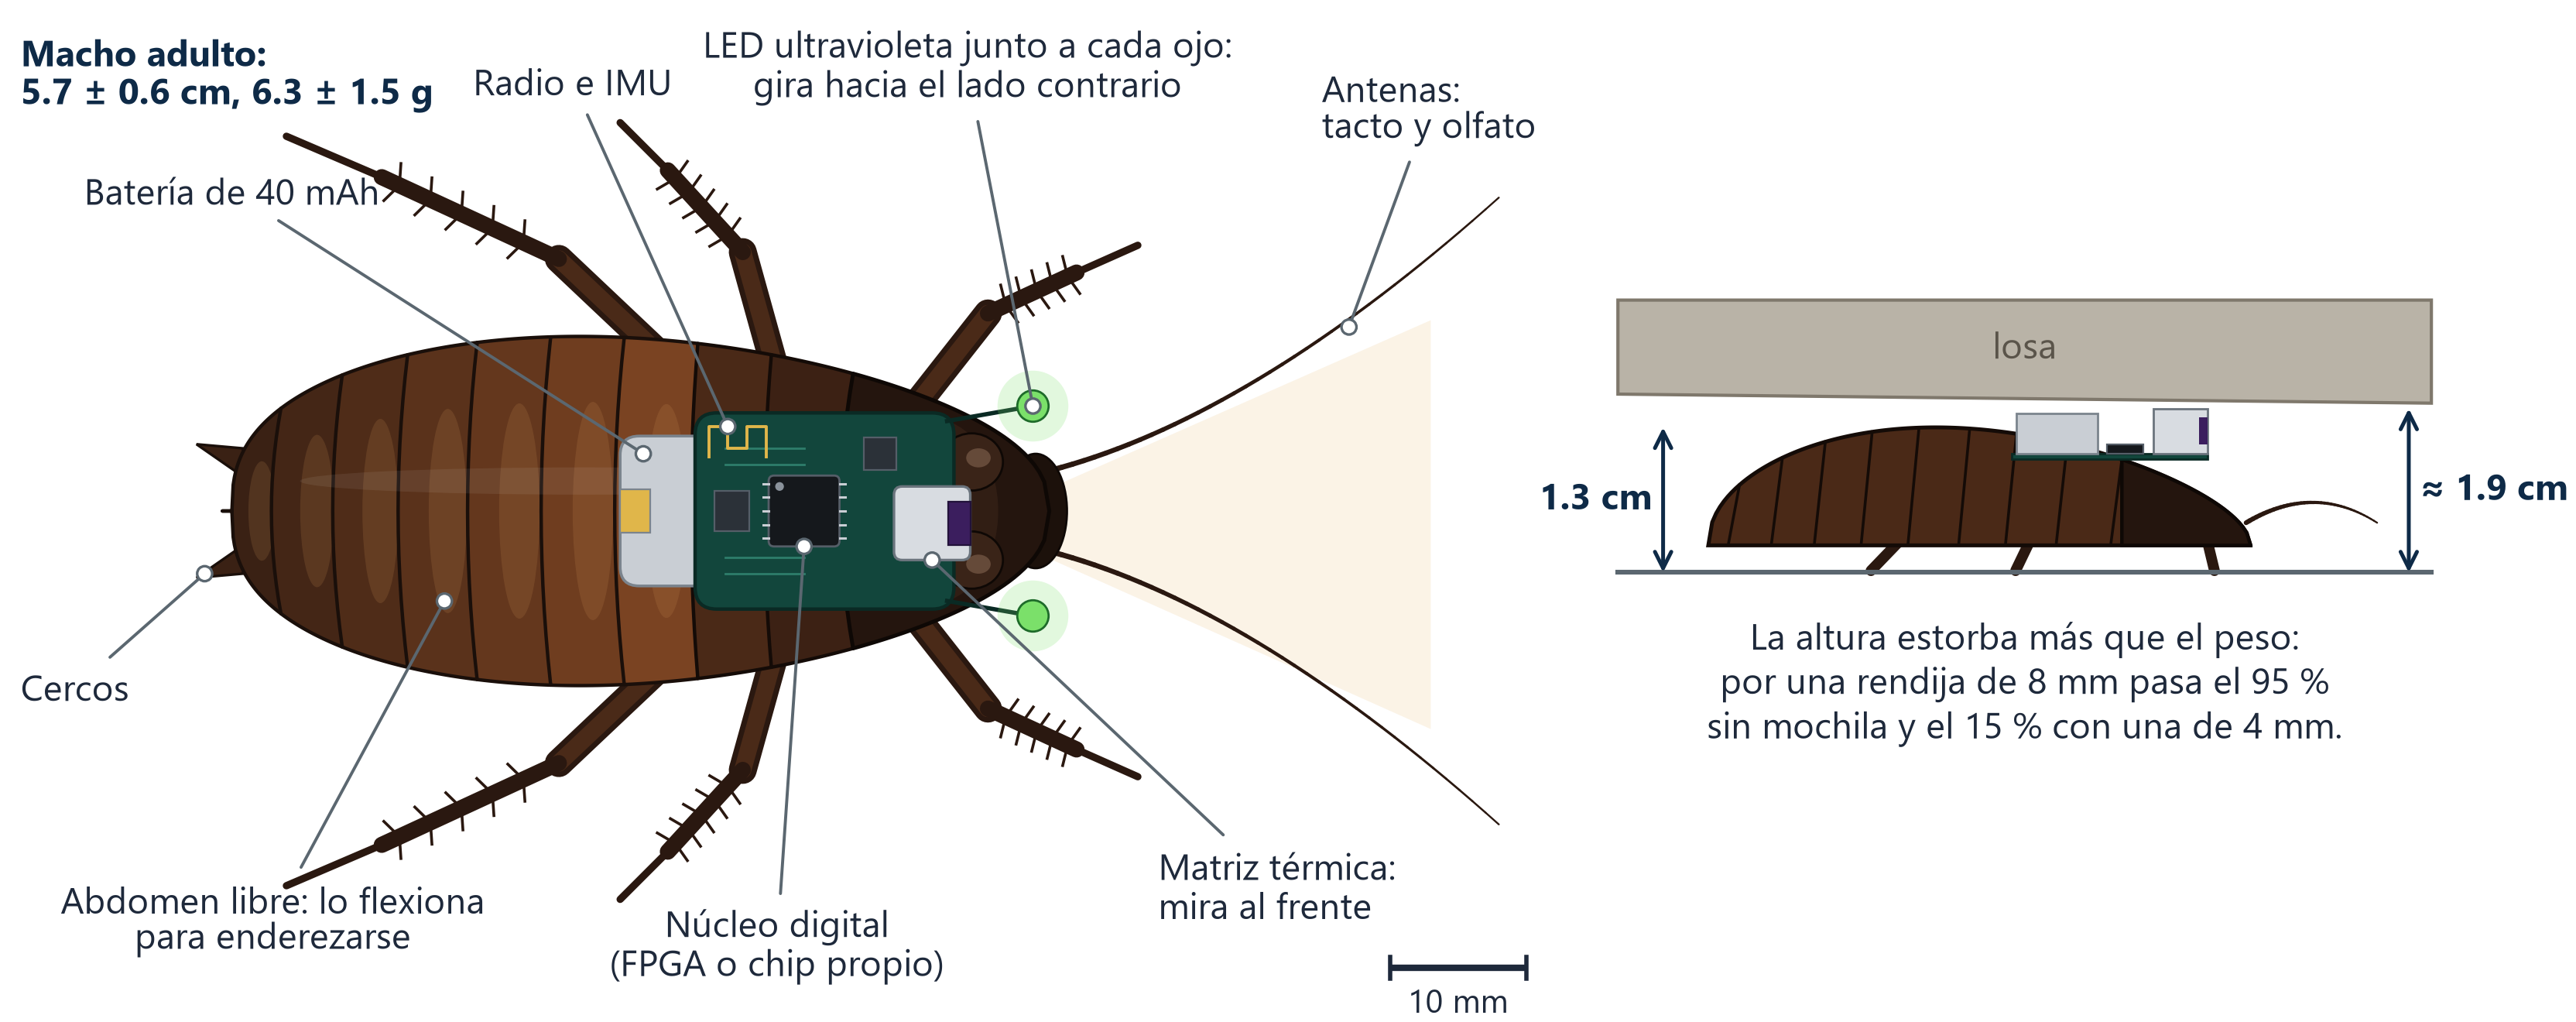
\includegraphics[width=0.96\textwidth]{figs/insecto_mochila.png}
\caption{\Gp{} con la mochila, a escala. Dibujo propio; medidas de~\cite{tranngoc2023,li2019} y paso por
rendijas de~\cite{kai2026}.}
\label{fig:insecto}
\end{figure}

\begin{table}[!htb]
\centering\footnotesize
\caption{Capacidades de \Gp{} y lo que implican para la mochila.}
\label{tab:capacidades}
\rowcolors{2}{SoftGray}{white}
\begin{tabularx}{\textwidth}{@{}>{\bfseries\raggedright\arraybackslash}p{2.0cm} >{\raggedright\arraybackslash}X >{\raggedright\arraybackslash}p{5.2cm}@{}}
\toprule
\rowcolor{TableHead} Capacidad & Dato publicado & Consecuencia de diseño \\
\midrule
Masa y tamaño & $6.32\pm1.5$~g y $5.7\pm0.6$~cm~\cite{tranngoc2023}; 2.2~cm de ancho, 1.3~cm de alto~\cite{li2019} & Mochila para un animal de 6~g \\
Carga & Con 15~g se detiene por completo~\cite{montagut2024}; con 4~g ya empeora el control~\cite{latif2012} & Meta de 2 a 3~g (30 a 45~\% de su masa) \\
Altura & Rendija de 8~mm: pasa el 95~\% sin mochila y el 15~\% con una de 4~mm~\cite{kai2026} & Componentes lado a lado, no apilados \\
Velocidad & 1.9~cm/s natural~\cite{dirafzoon2017}; 3.7 a 5.0~cm/s guiada~\cite{tranngoc2024} & El modelo usa 1.9 y 5~cm/s (4~s por estímulo) \\
Pausas & Quieta cerca del 60~\% del tiempo, 37~s por pausa~\cite{dirafzoon2017} & La política debe reiniciar la marcha \\
Enderezarse & 98~\% sin carga; 31 a 69~\% con mochila~\cite{li2019,montagut2024} & Mochila baja y ligera \\
Temperatura & Actividad máxima cerca de 30~\textdegree C; a 34 y 38~\textdegree C inmóvil más de la mitad del tiempo~\cite{gracidas2026} & Ventana de operación de 22 a 30~\textdegree C \\
Energía & 5~mW en reposo, 17 a 31~mW caminando (calculado de~\cite{herreid1981}) & La locomoción la paga el insecto \\
\bottomrule
\end{tabularx}
\end{table}

Esta revisión nos obligó a corregir cuatro cifras de nuestra propuesta inicial, y algunas por mucho. Habíamos puesto 15~g de
carga útil y quedó en 2--3~g. La velocidad pasó de 0.3~m/s a 1.9--5~cm/s. El umbral térmico fijo de 35.5--38.5~\textdegree C
tampoco servía, porque es la temperatura central del cuerpo y lo que ve el sensor es la piel. Y el circuito, que calculábamos en
60 celdas, resultó de 477 elementos lógicos.

\textbf{Masa y energía.} Elegimos una matriz térmica, un radio de baja potencia, una IMU y una batería de 40~mAh, que
juntos pesan unos 2.9~g (figura~\ref{fig:presupuestos}). Con el sensor encendido el consumo es de cerca de 30~mW, y de ahí
estimamos una autonomía de $t=0.85\times40~\text{mAh}\times3.7~\text{V}/30~\text{mW}\approx4$~h. Como referencia medida, la
mochila de NTU gasta 205.5~mW y dura 2.2~h con 120~mAh~\cite{tranngoc2023}. El cómputo casi no pesa: una iCE40 UltraLite de
1\,248 LUT mide $1.4\times1.4$~mm y pesa unos 2~mg~\cite{lattice}, y el nRF52840 anda por los 15~mg~\cite{nordic}. Por eso
preferimos gastar lógica, que no agrega masa, con tal de ahorrar energía y estímulos.

\begin{figure}[!htb]
\centering
\begin{subfigure}{0.48\textwidth}
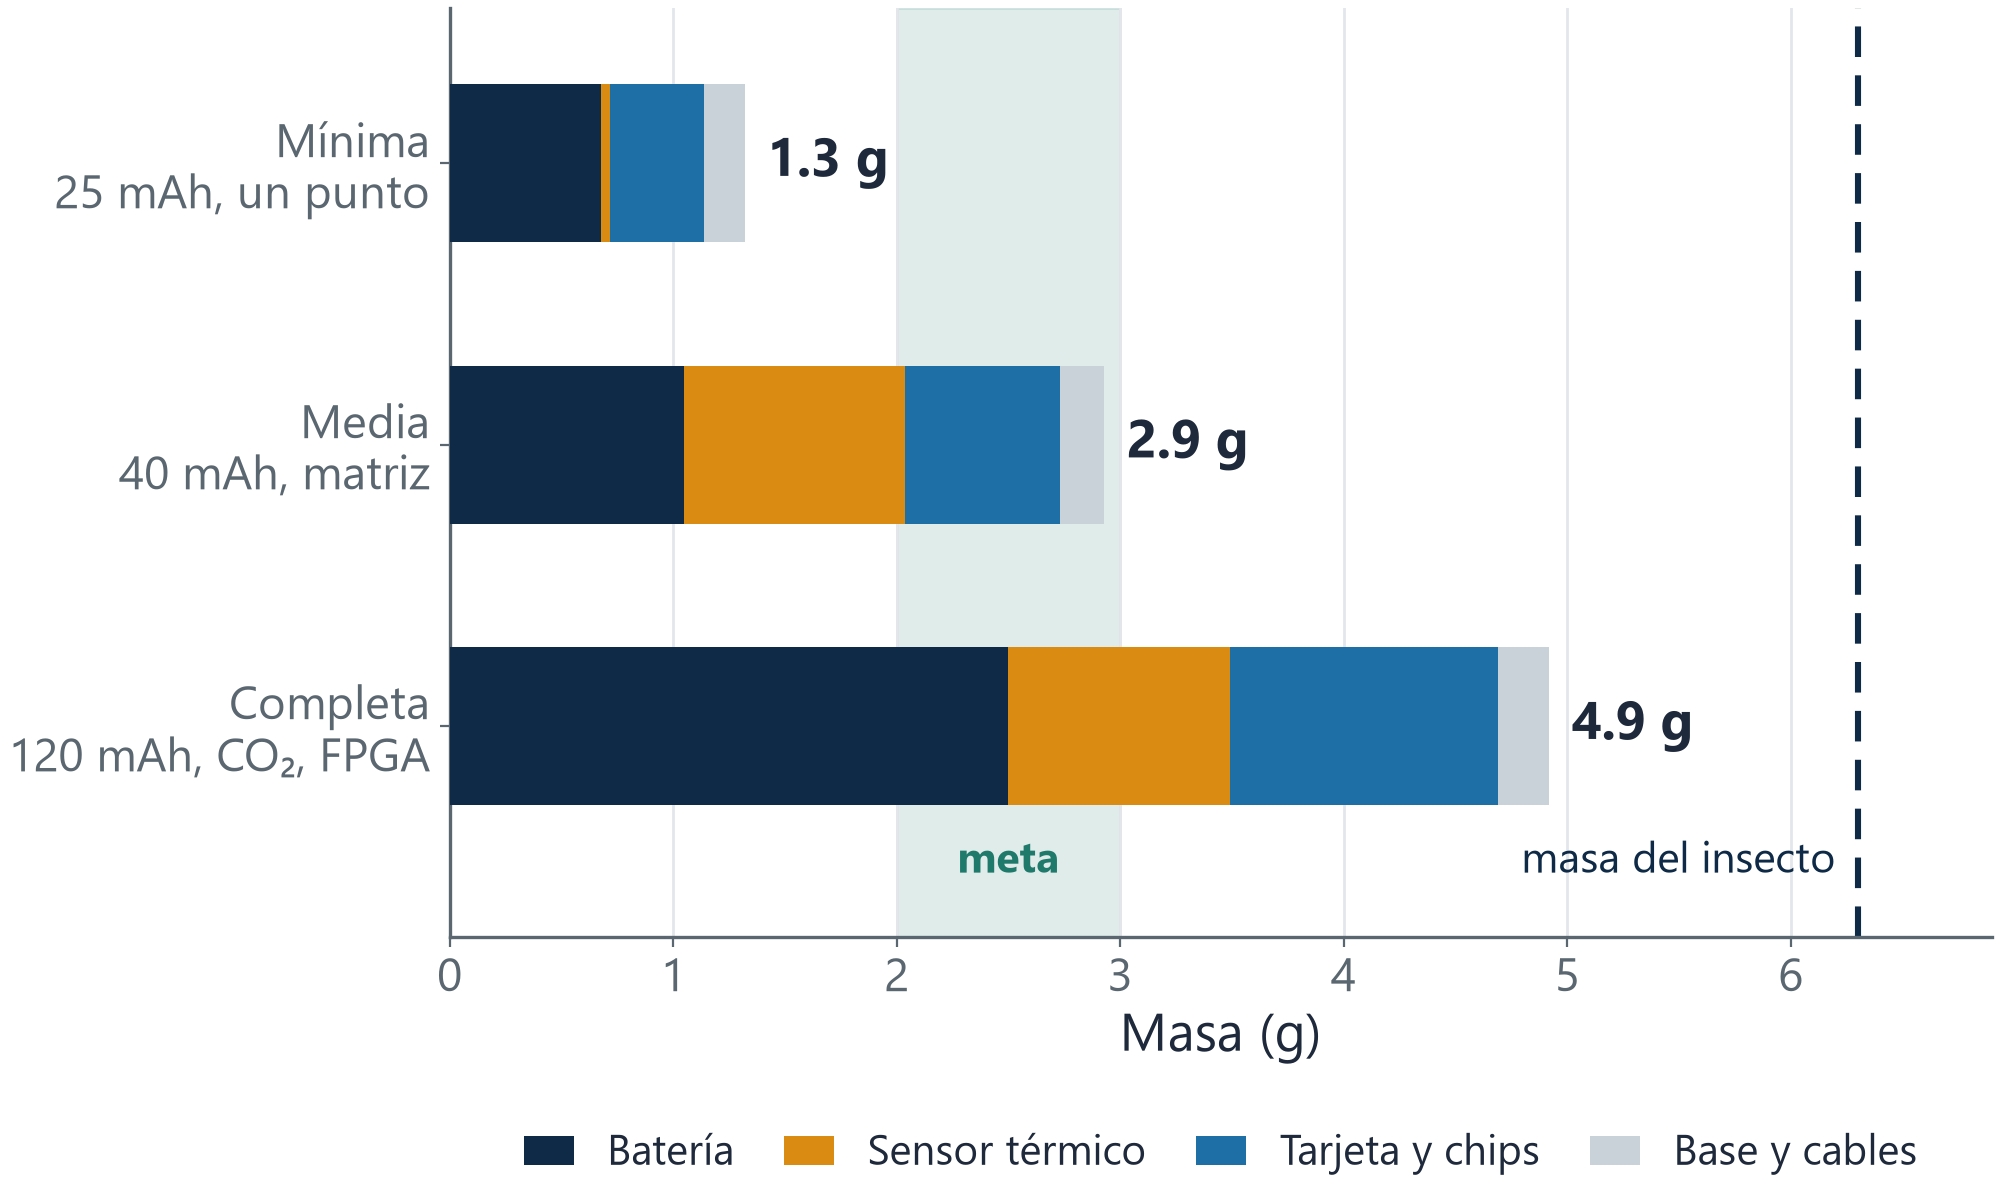
\includegraphics[width=\linewidth]{figs/presupuesto_masa.png}
\caption{Masa por configuración.}
\end{subfigure}\hfill
\begin{subfigure}{0.48\textwidth}
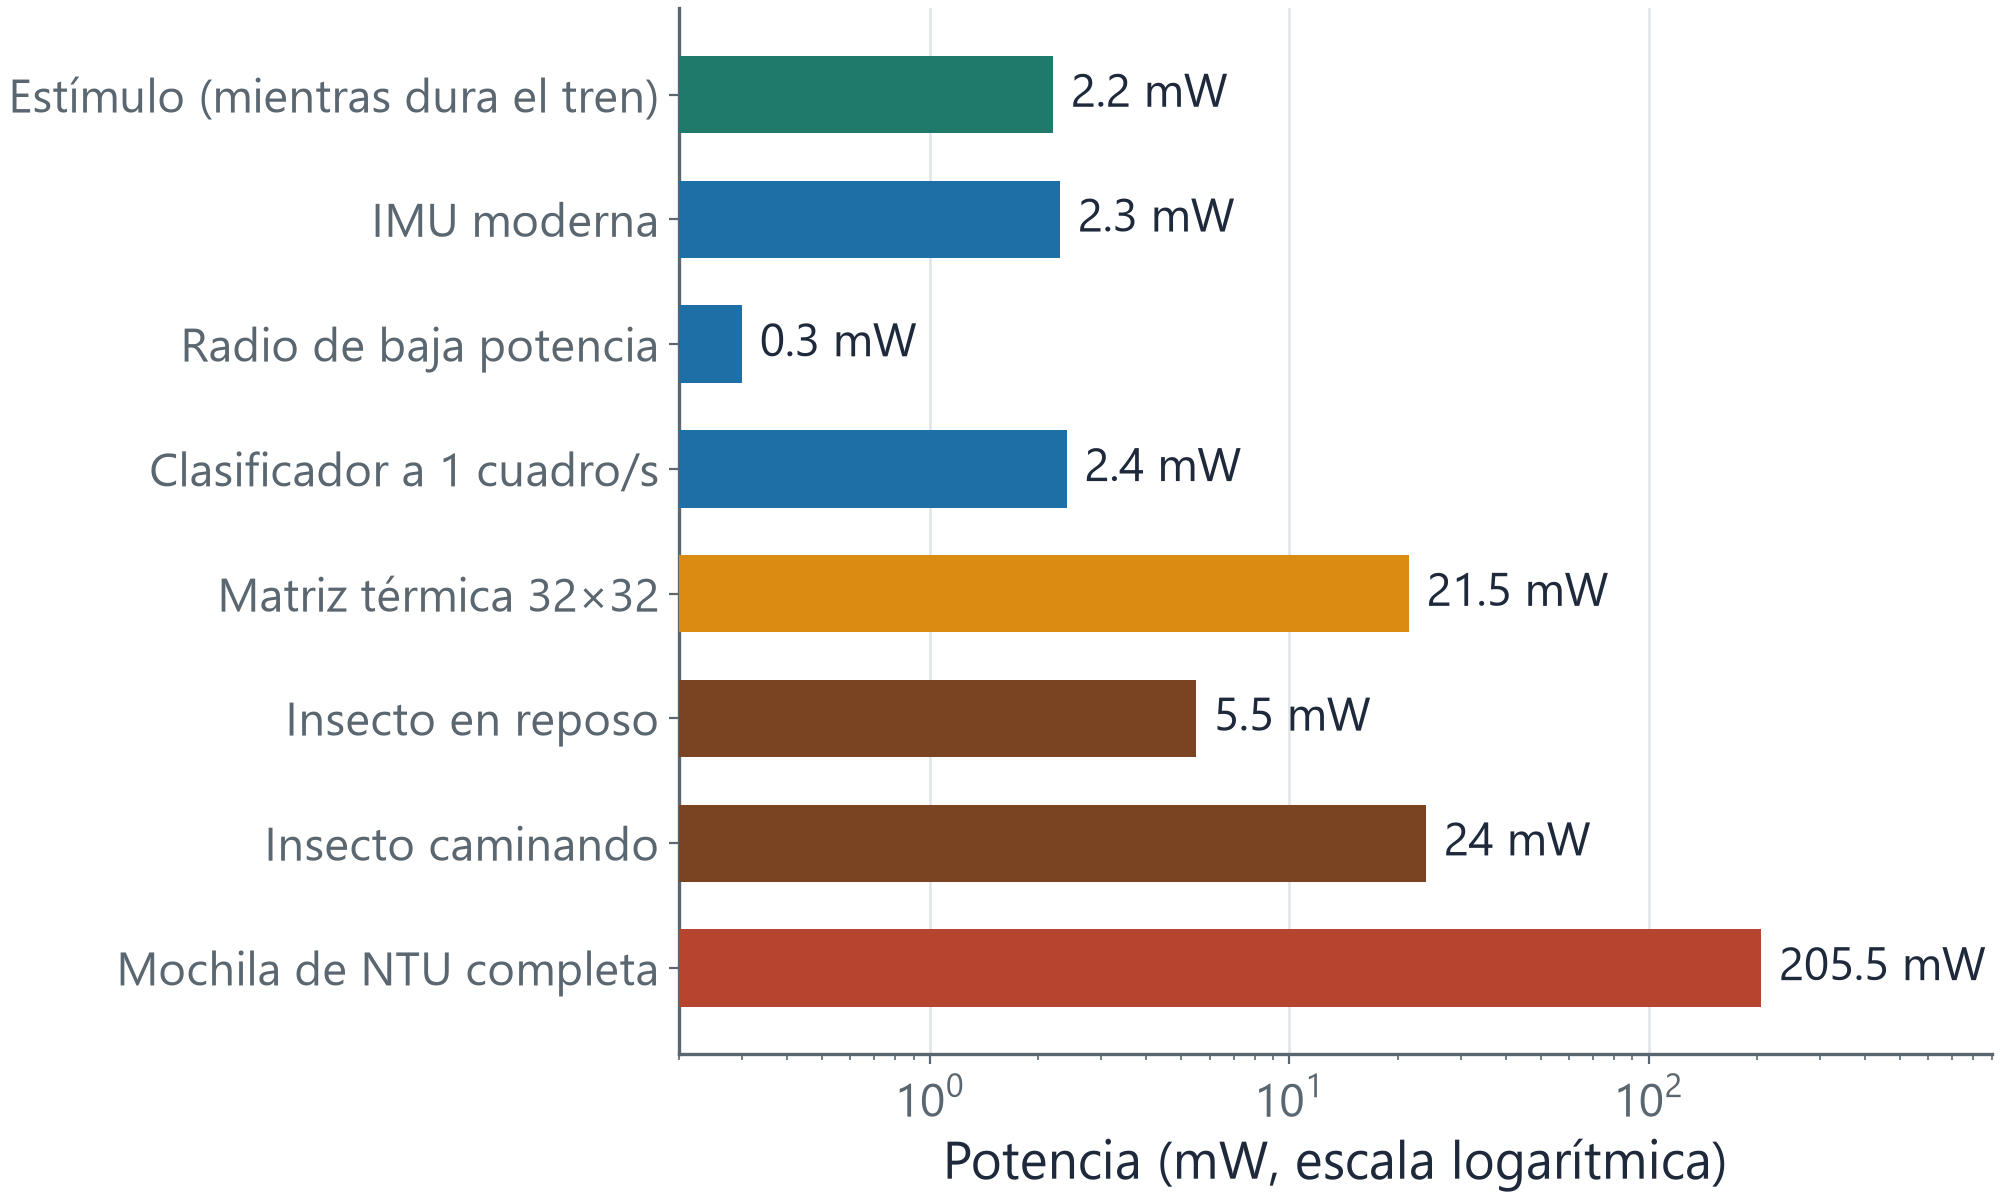
\includegraphics[width=\linewidth]{figs/energia.png}
\caption{Quién gasta qué.}
\end{subfigure}
\caption{Presupuestos de la mochila. Masas de batería y sensor medidas~\cite{tranngoc2023}; las de los chips
son estimadas.}
\label{fig:presupuestos}
\end{figure}

\subsection{El modelo de la misión}
\label{sec:modelo}

\textbf{Marcha.} Para el insecto sin estímulo usamos el modelo de Dirafzoon et al.~\cite{dirafzoon2017} con los valores de
Tran-Ngoc et al.~\cite{tranngoc2024}. Camina en tramos rectos exponenciales de media $l^*=17.6$~cm a $v=1.94$~cm/s. Al
terminar cada tramo puede detenerse, con probabilidad $P_s=0.211$, un tiempo medio $T_s=36.8$~s, y si va siguiendo una pared
solo la suelta con probabilidad $p_e=0.005$. Con eso se obtiene la fracción del tiempo que camina,
\begin{equation}
F_m=\frac{l^*/v}{l^*/v+P_s\,T_s}=\frac{9.1}{9.1+7.8}=0.54 ,
\end{equation}
dentro del intervalo medido de $0.37\pm0.20$.

\textbf{Estímulo.} Nos quedamos con la luz ultravioleta. No requiere cirugía, no se ha observado habituación en 150
ensayos~\cite{refat2025} y la colonia de la universidad responde a ella~\cite{gracidas2026}. Como alternativa dejamos los
electrodos de superficie~\cite{lin2023,tranngoc2025} (81~\% y 74~\% de éxito), ya que el generador de pulsos sirve para los
dos. En la tabla~\ref{tab:estimulos} comparamos las opciones. En el modelo, el insecto obedece con probabilidad $p\,(1-H)$,
con $p=0.78$~\cite{lin2023}; la habituación $H$ sube con cada estímulo y baja con el descanso:
\begin{equation}
H\leftarrow H+\alpha\,(1-H) \quad\text{por estímulo},\qquad H(t+\Delta t)=H(t)\,e^{-\Delta t/\tau}.
\end{equation}
Con $\tau=600$~s~\cite{sanchez2015} y $\alpha=0.09$ el modelo reproduce bien los datos de pulsos unipolares. Tras diez estímulos, uno cada 15~s, queda el 46~\% de la respuesta (medido:
43~\%~\cite{ma2023}), y tras cuarenta, el 22~\% (medido: 20~\%~\cite{erickson2015}). Con onda bifásica o con luz, $\alpha$
es al menos cuarenta veces menor (figura~\ref{fig:habituacion}). En la simulación usamos $\alpha=0.01$, que es un valor
conservador.

\begin{figure}[!htb]
\centering
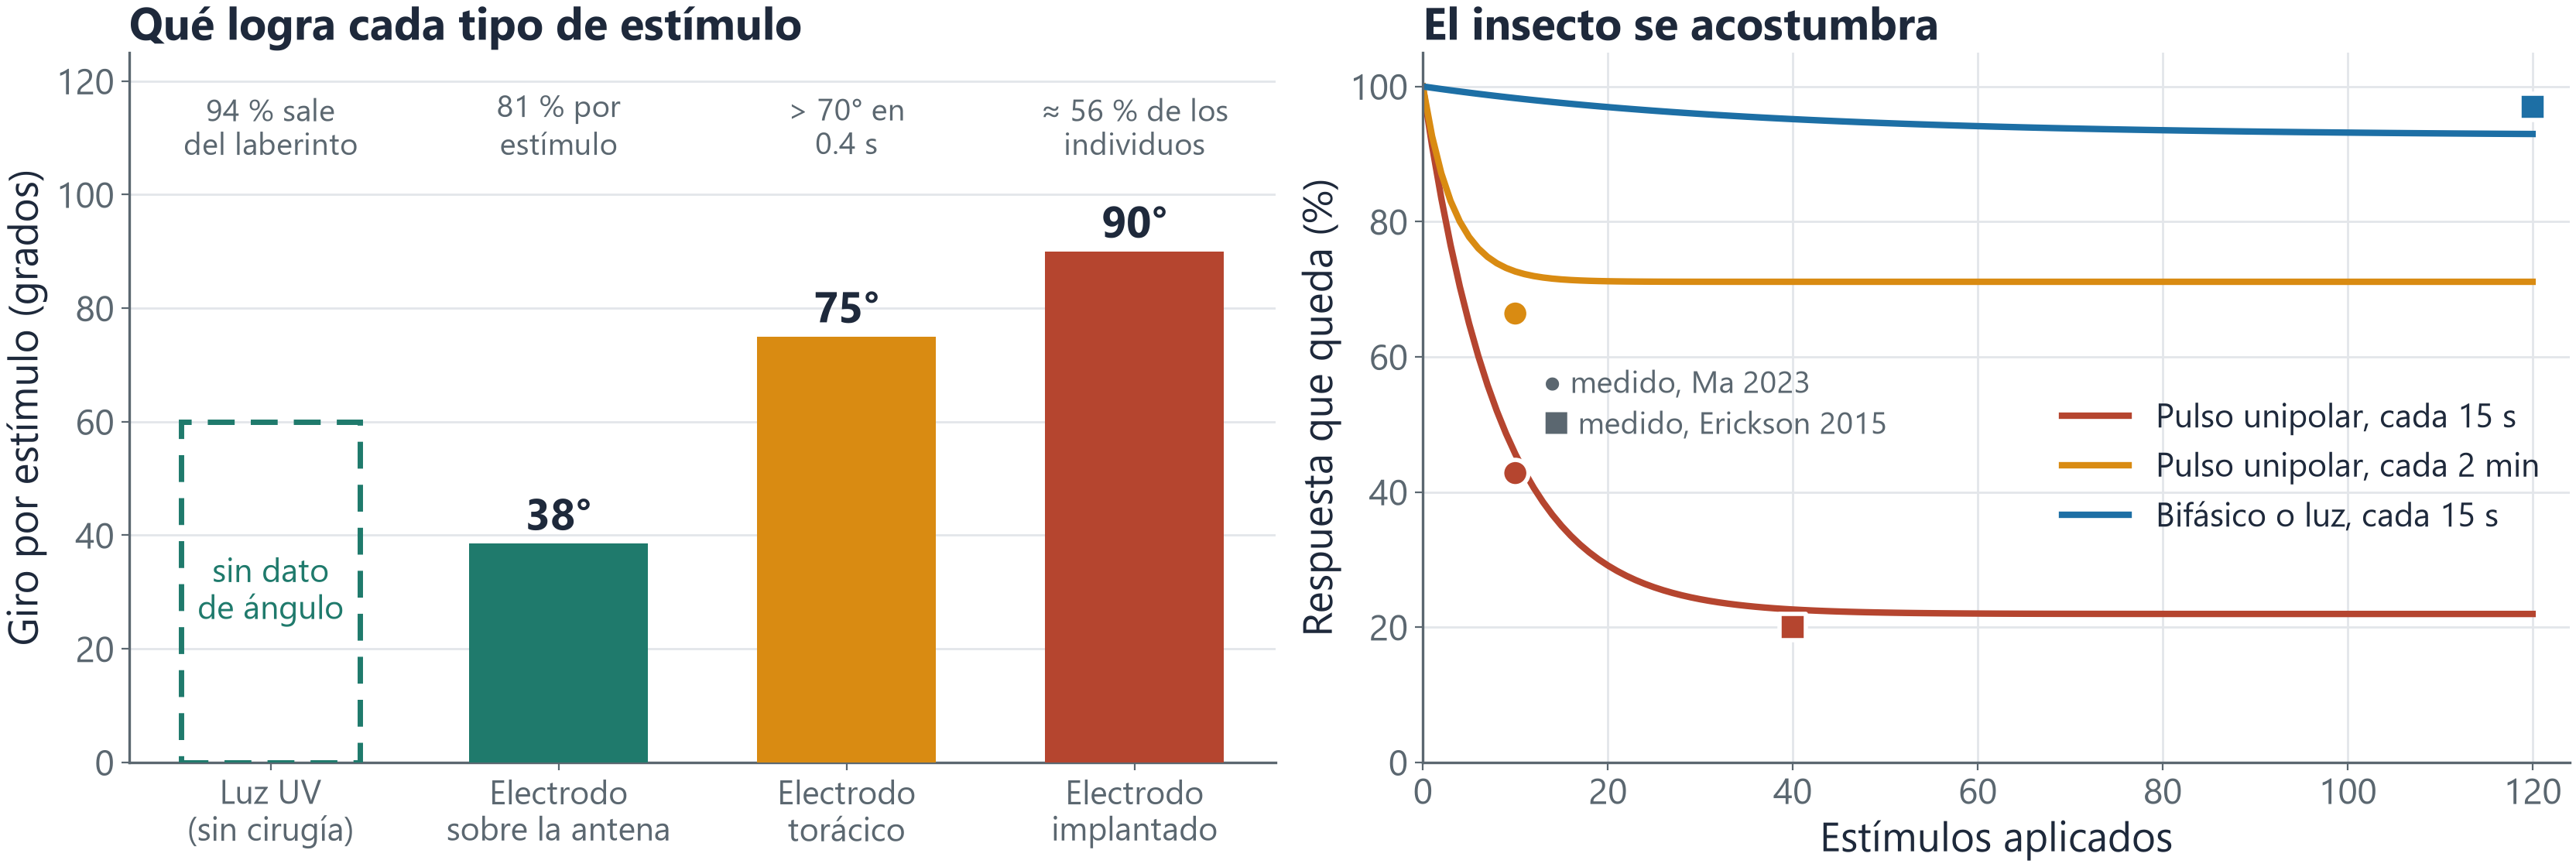
\includegraphics[width=0.96\textwidth]{figs/habituacion.png}
\caption{Izquierda: giro por estímulo según el método~\cite{lin2023,lin2025,ma2023}. Derecha: modelo de
habituación frente a los datos medidos.}
\label{fig:habituacion}
\end{figure}

\begin{table}[!htb]
\centering\footnotesize
\caption{Tipos de estímulo para dirigir a \Gp.}
\label{tab:estimulos}
\rowcolors{2}{SoftGray}{white}
\begin{tabularx}{\textwidth}{@{}>{\bfseries\raggedright\arraybackslash}p{4.0cm} >{\raggedright\arraybackslash}p{1.4cm} >{\raggedright\arraybackslash}X >{\raggedright\arraybackslash}X@{}}
\toprule
\rowcolor{TableHead} Estímulo & Cirugía & Eficacia publicada & Inconveniente \\
\midrule
Electrodo en la antena~\cite{latif2012,erickson2015} & Sí & 56~\% de los individuos & Inutiliza la antena; dura días \\
Electrodo en los cercos~\cite{tranngoc2023} & Sí & 94~\% de navegaciones & El sentido del giro varía \\
Electrodo torácico~\cite{lin2025} & Poca & Giro de más de 70\textdegree{} en 0.4~s & Ensamble preciso \\
Electrodo de superficie~\cite{lin2023,tranngoc2025} & No & 81~\% y 74~\% por estímulo & Impedancia de 70 a 123~k$\Omega$ \\
Luz ultravioleta~\cite{refat2025,gracidas2026} & No & Sin habituación en 150 ensayos & Falta medir el ángulo por pulso \\
\bottomrule
\end{tabularx}
\end{table}

\textbf{Detección.}\phantomsection\label{sec:deteccion} Lo primero fue ver si bastaba un sensor de un solo píxel. El problema es que promedia todo su campo $\varphi$. Si el blanco tiene
un área $A$ y está a una distancia $d$, llena la fracción $f$ y la lectura es
\begin{equation}
T_{\text{leída}}=T_f+f\,(T_p-T_f),\qquad f=\min\!\left(1,\ \frac{A}{\pi\,d^2\tan^2(\varphi/2)}\right).
\end{equation}
Con una cara ($0.03$~m$^2$) a 33~\textdegree C sobre un fondo de 22~\textdegree C y $\varphi=90$\textdegree, a
medio metro se leen 22.4~\textdegree C. Es decir, con un solo píxel prácticamente no se nota que hay una persona. Con una matriz sí, porque cada píxel ve un ángulo
$\theta$ y el blanco ocupa $n=A/(d\tan\theta)^2$ píxeles. El núcleo cuenta como caliente el píxel que está entre 28 y
38~\textdegree C, que es el criterio de NTU~\cite{tranngoc2023}, y le agregamos que además esté 2~\textdegree C por encima de
la media del cuadro anterior. Con 2 píxeles empieza a acercarse y con 8 durante cuatro cuadros seguidos declara la detección
(figura~\ref{fig:deteccion}). La matriz de $8\times8$ (AMG8833~\cite{panasonic}, 599~MXN~\cite{unit}) confirma a 0.9~m y la de
$32\times24$ (MLX90640~\cite{melexis}, 1\,100~MXN), a 2.0~m.

\begin{figure}[!htb]
\centering
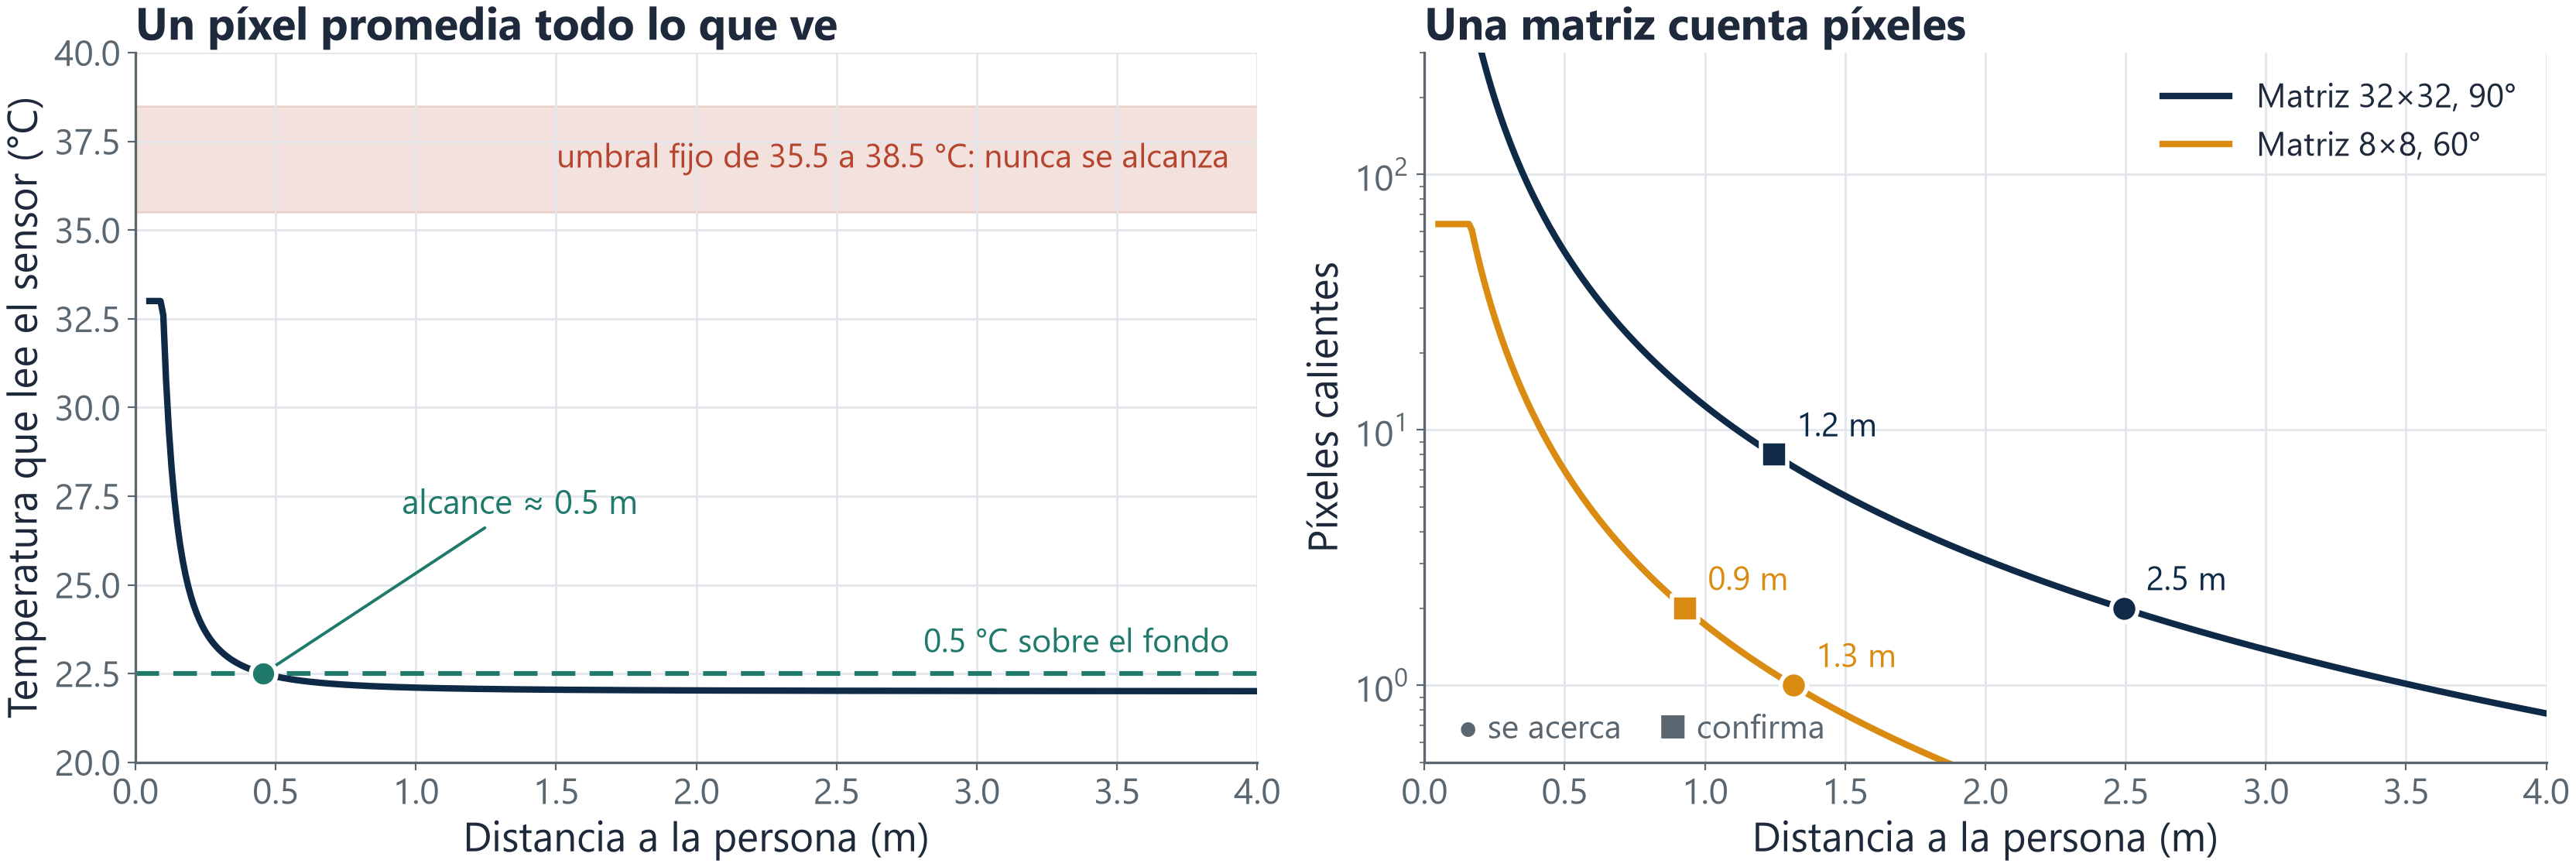
\includegraphics[width=0.98\textwidth]{figs/deteccion_termica.png}
\caption{Izquierda: lectura de un píxel de 90\textdegree{} frente a la distancia. Derecha: píxeles calientes con
dos matrices; el círculo marca el acercamiento y el cuadro, la confirmación.}
\label{fig:deteccion}
\end{figure}

\textbf{Límites físicos.} Arriba de unos 30~\textdegree C se pierde el contraste con la piel y además el insecto deja de
moverse (figura~\ref{fig:limites}). Para esos casos harían falta otras señales, como el CO$_2$ que exhala la
persona~\cite{huo2011} o el sonido. El concreto atenúa unos 22~dB por metro a 915~MHz y 47~dB a
2.4~GHz~\cite{itu2040,stone1997}, así que la radio tiene que ser de menos de 1~GHz y con un relevo en el boquete.

\begin{figure}[!htb]
\centering
\begin{subfigure}{0.47\textwidth}
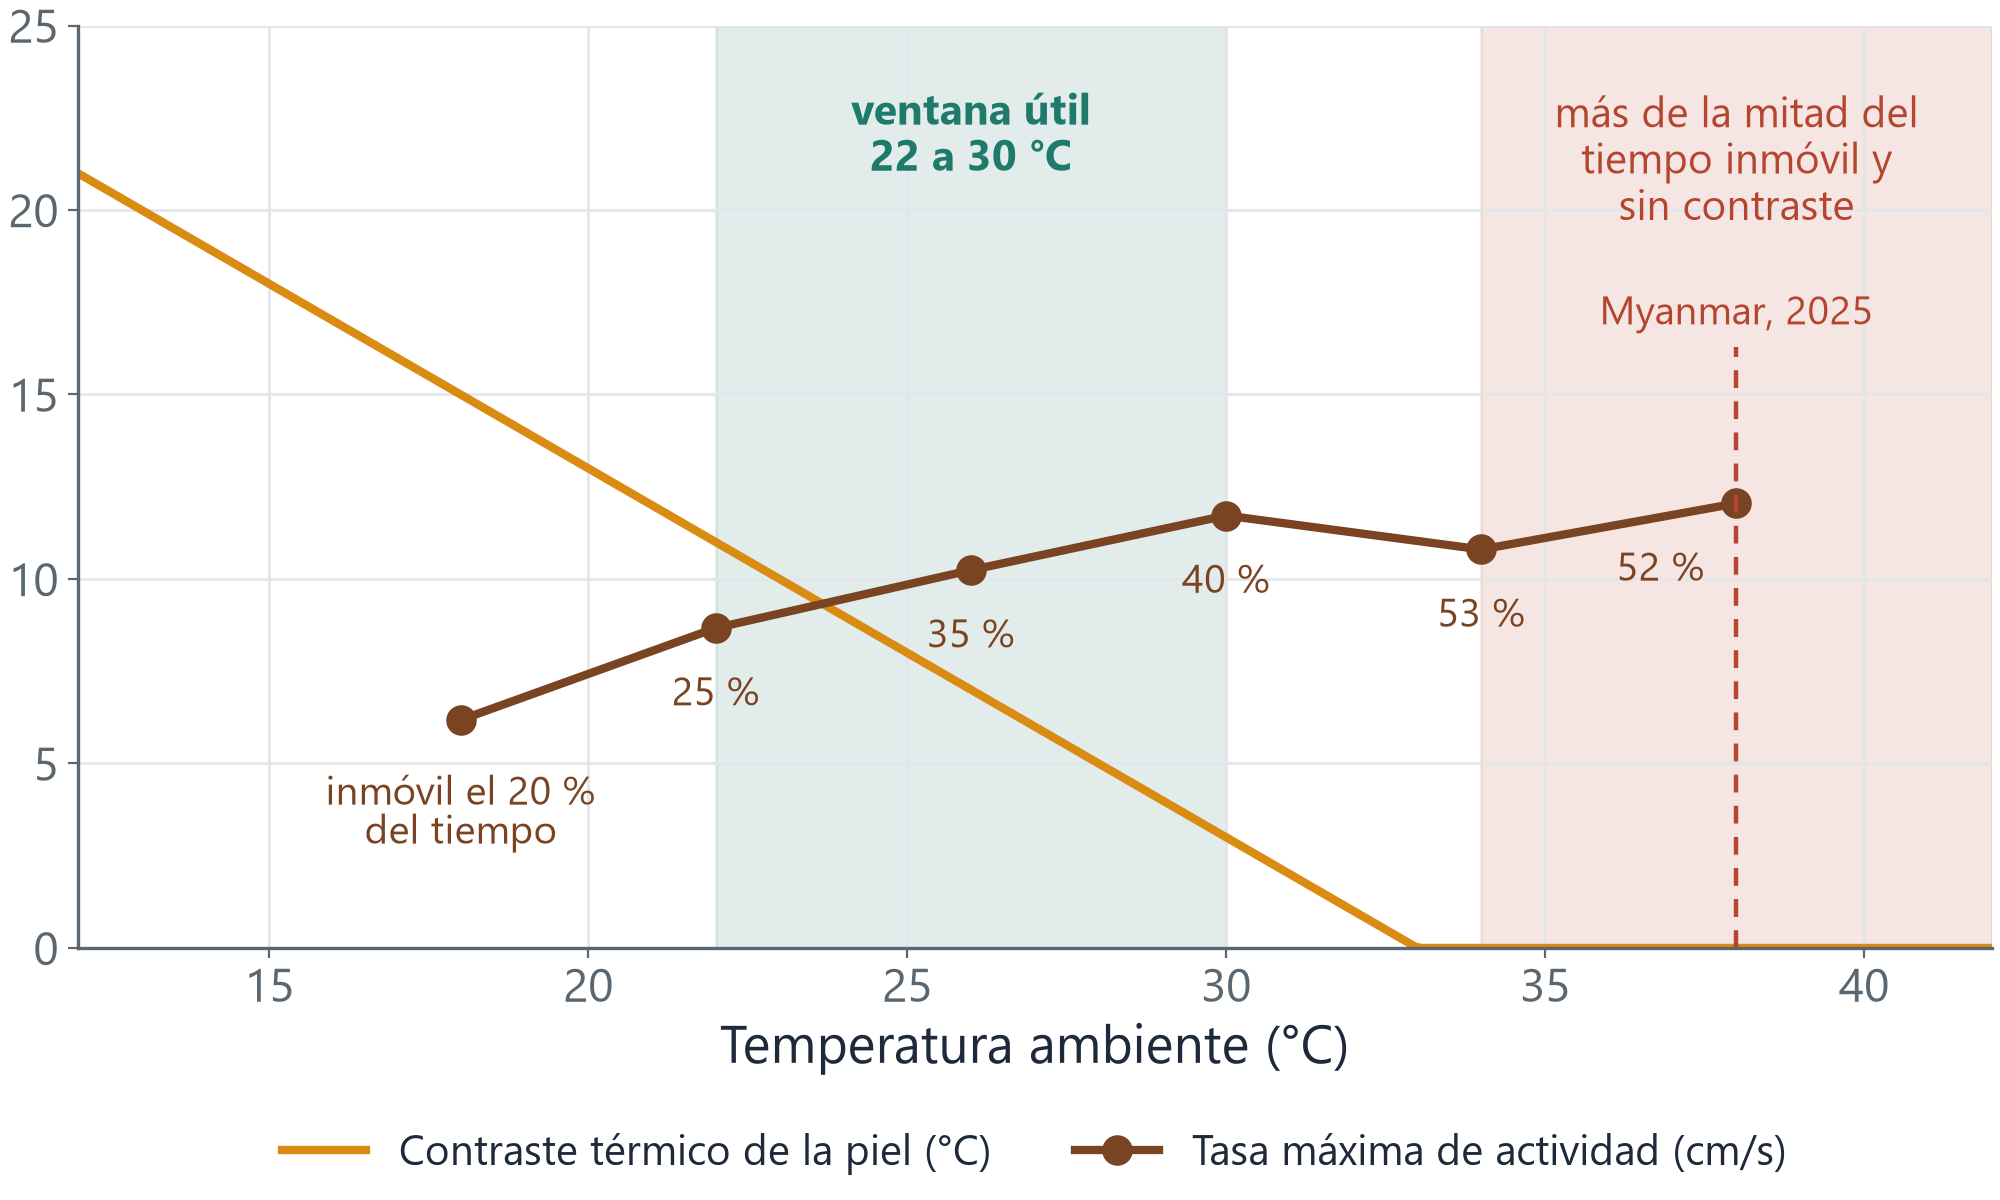
\includegraphics[width=\linewidth]{figs/ventana_operativa.png}
\caption{Ventana de temperatura.}
\end{subfigure}\hfill
\begin{subfigure}{0.47\textwidth}
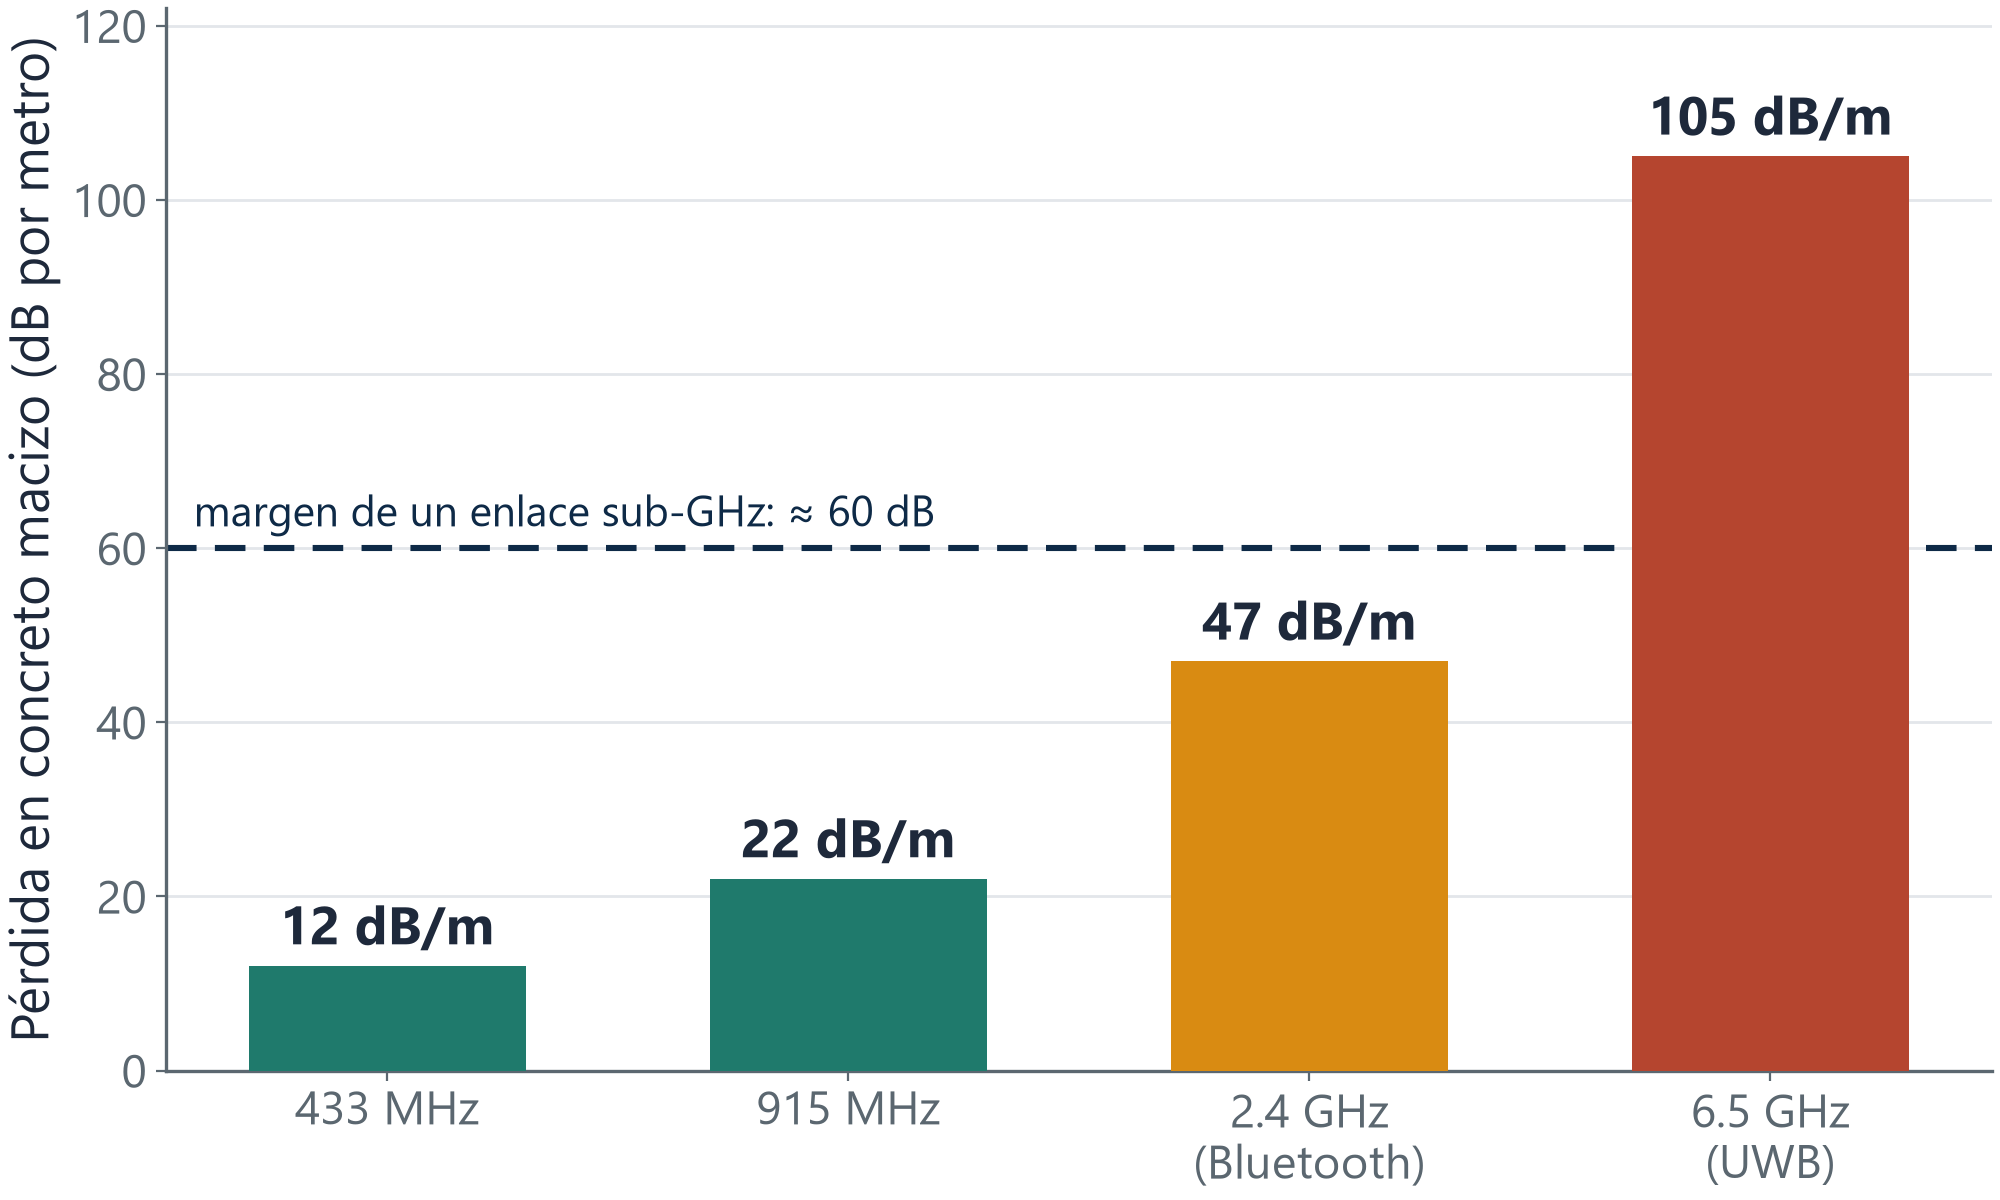
\includegraphics[width=\linewidth]{figs/radio_escombro.png}
\caption{Pérdida de la radio en concreto.}
\end{subfigure}
\caption{(a) Contraste térmico disponible y actividad del insecto~\cite{gracidas2026}. (b) Atenuación con el
modelo de la UIT~\cite{itu2040}.}
\label{fig:limites}
\end{figure}

\textbf{Localización y misión.} La alerta indica por qué boquete entró el insecto. La IMU estima cuánto caminó, con un
error de 5 a 10~\% de la distancia~\cite{tranngoc2024}, y para el último medio metro se usa una baliza. Simulamos la misión
con agentes en colapsos sintéticos de $8\times6$~m y tomamos como referencia analítica la teoría de búsqueda, que da
$P_d=1-e^{-C}$ con $C=W v t N/A_h$~\cite{frost2001}. Los parámetros que usamos están en la tabla~\ref{tab:parametros}.

\begin{table}[!htb]
\centering\footnotesize
\caption{Parámetros de la simulación. F: publicado; D: decisión de diseño; S: supuesto que se explora en la
sensibilidad.}
\label{tab:parametros}
\rowcolors{2}{SoftGray}{white}
\setlength{\tabcolsep}{4pt}
\begin{tabularx}{\textwidth}{@{}>{\raggedright\arraybackslash}X l l | >{\raggedright\arraybackslash}X l l@{}}
\toprule
\rowcolor{TableHead} \textbf{Parámetro} & \textbf{Valor} & & \textbf{Parámetro} & \textbf{Valor} & \\
\midrule
Velocidad natural & $1.94\pm0.29$~cm/s & F~\cite{dirafzoon2017} & Recuperación, $\tau$ & 600~s & F~\cite{sanchez2015} \\
Tramo recto, media & 17.6~cm & F~\cite{dirafzoon2017} & Espera antes de reactivar & 15~s, hasta $\times8$ & D \\
Pausa por tramo & 0.211 & F~\cite{dirafzoon2017} & Mínimo entre estímulos & 10~s & D \\
Duración de la pausa & $36.8\pm24.1$~s & F~\cite{dirafzoon2017} & Giros al azar & cada 51~s & D \\
Soltar la pared & 0.005 & F~\cite{dirafzoon2017} & Presupuesto & 12; $\tau=600$~s & D \\
Obedece un estímulo & 0.78 & F~\cite{lin2023} & Píxeles: acercar, confirmar & 2 y 8 & D \\
Giro por estímulo & $52\pm23$\textdegree & F~\cite{lin2023,ma2023} & Piel a la vista & 0.03~m$^2$ & S \\
Avance & 5~cm/s, 4~s & F~\cite{tranngoc2024} & Dobla esquinas & 0.80 & S \\
Habituación, $\alpha$ & 0.01 & F~\cite{erickson2015} & Insectos perdidos por hora & 0 & S \\
\bottomrule
\end{tabularx}
\end{table}

\subsection{El núcleo de la mochila, módulo por módulo}
\label{sec:nucleo}

La mochila deja que el insecto explore solo y estimula lo mínimo. La política es una máquina de ocho estados que
avanza una vez por cuadro térmico, diez veces por segundo (figura~\ref{fig:fsm}), y tres reglas la distinguen de
un control remoto: la espera que se duplica si el insecto no responde, los giros al azar que lo despegan de las
paredes~\cite{dirafzoon2017} y un presupuesto que limita los estímulos. La figura~\ref{fig:nucleo} muestra los
módulos; el recuadro punteado es lo que iría en el chip. En cada encabezado van el archivo y los elementos
lógicos (EL) y registros (R) que reporta Quartus.

\begin{figure}[!htb]
\centering
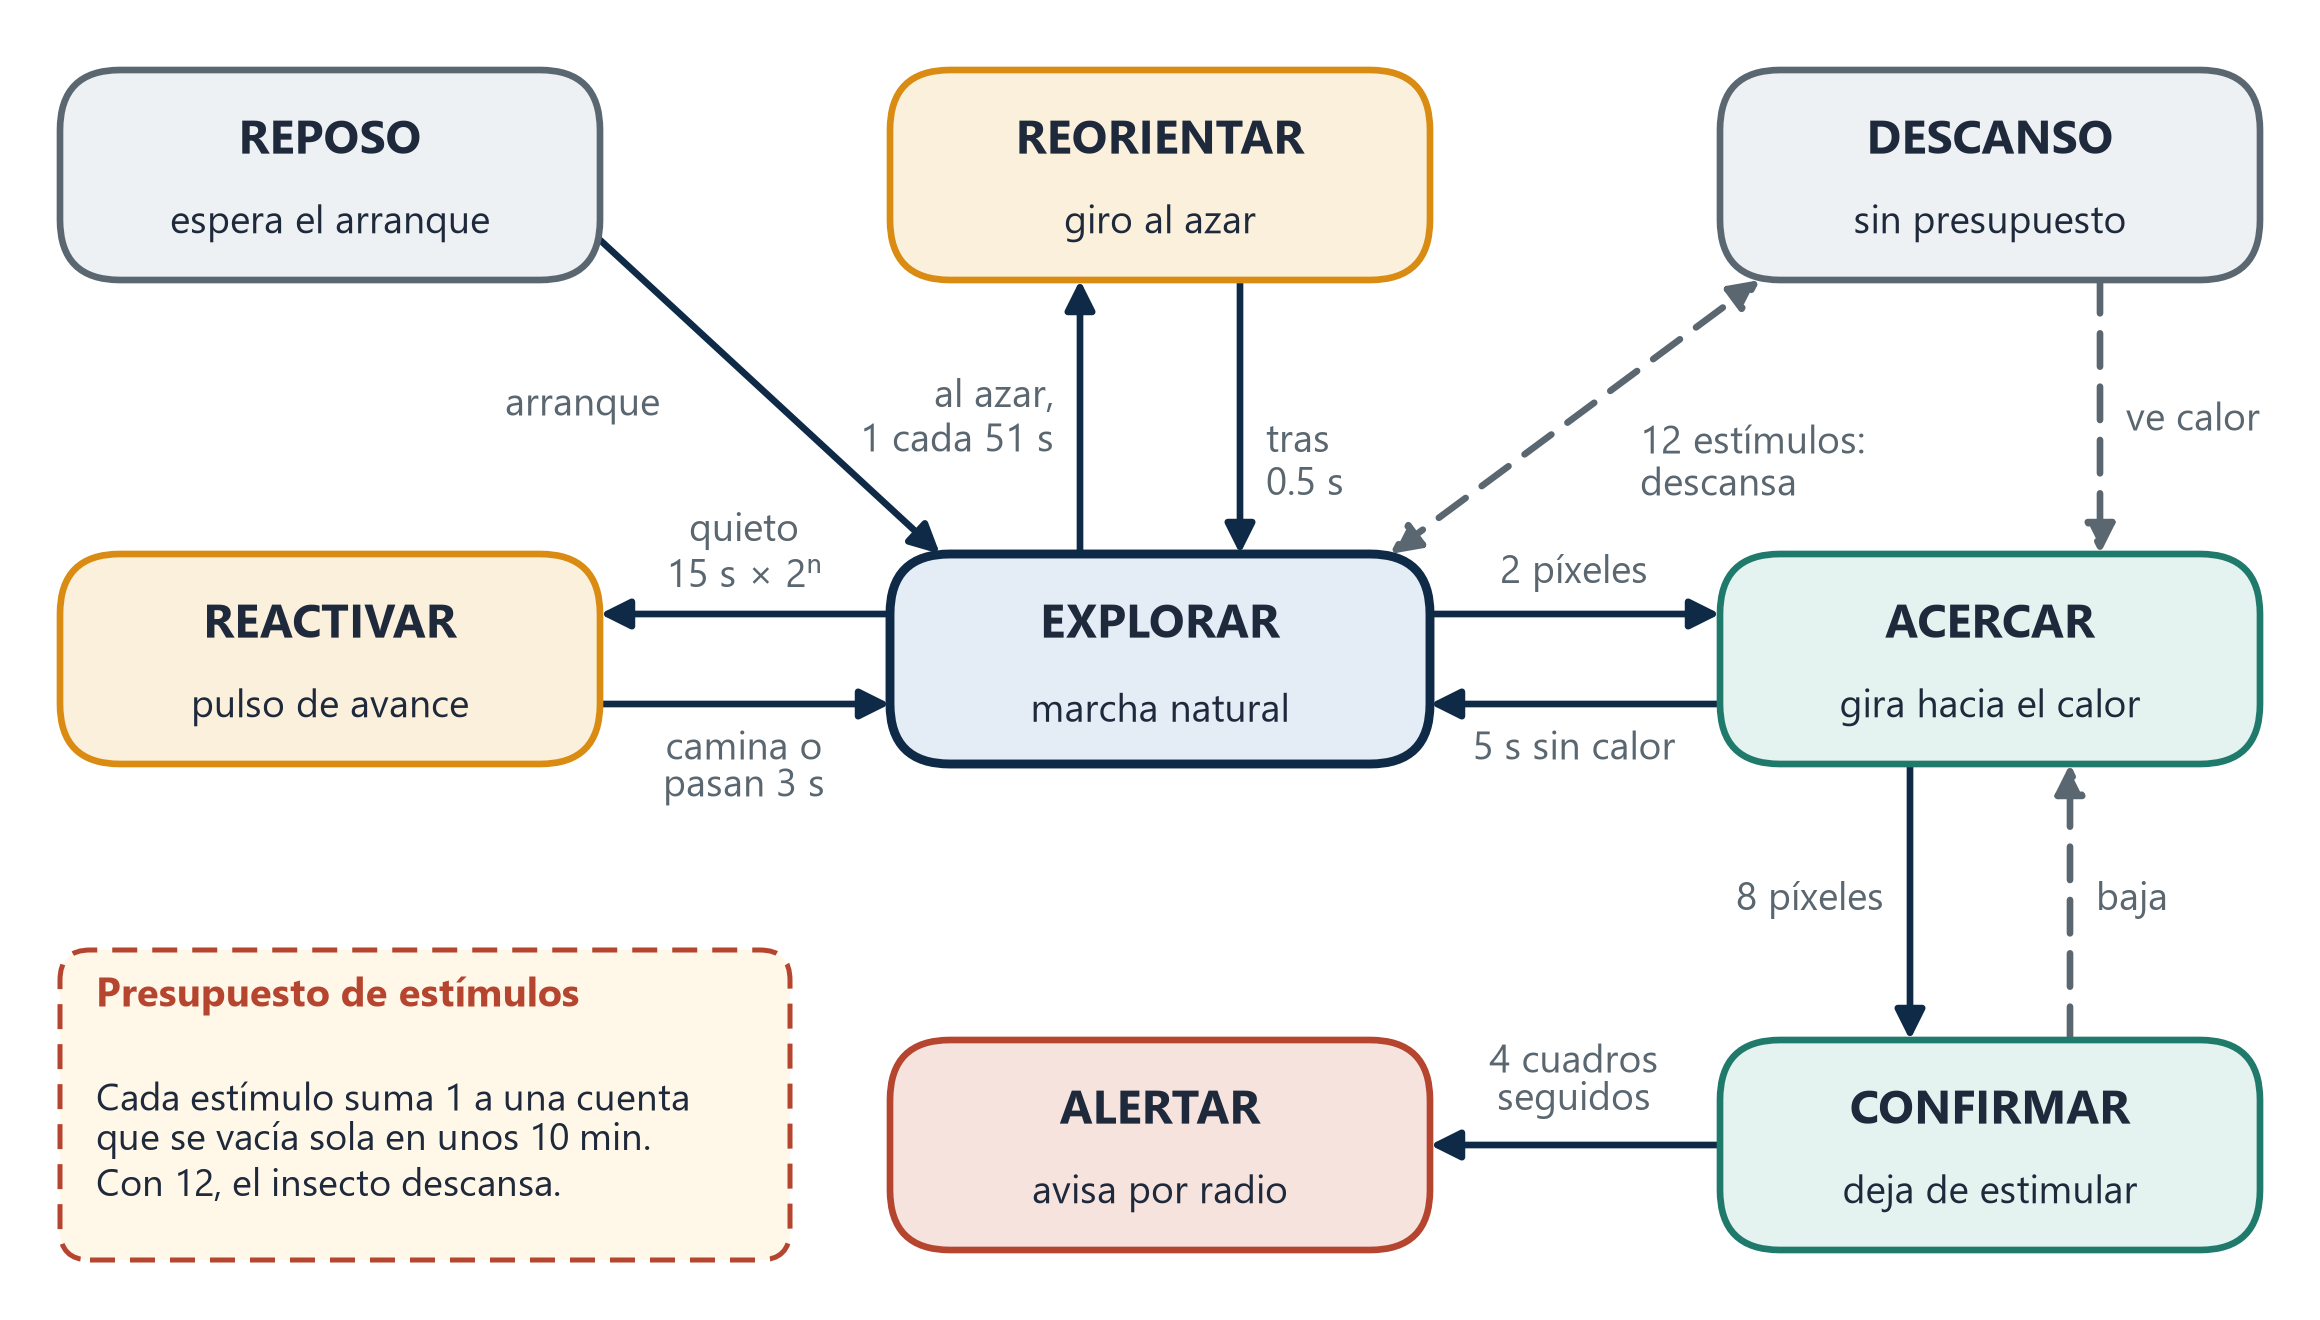
\includegraphics[width=0.80\textwidth]{figs/fsm_politica.png}
\caption{Máquina de estados de la política. Las flechas punteadas no producen estímulo.}
\label{fig:fsm}
\end{figure}

\begin{figure}[!htb]
\centering
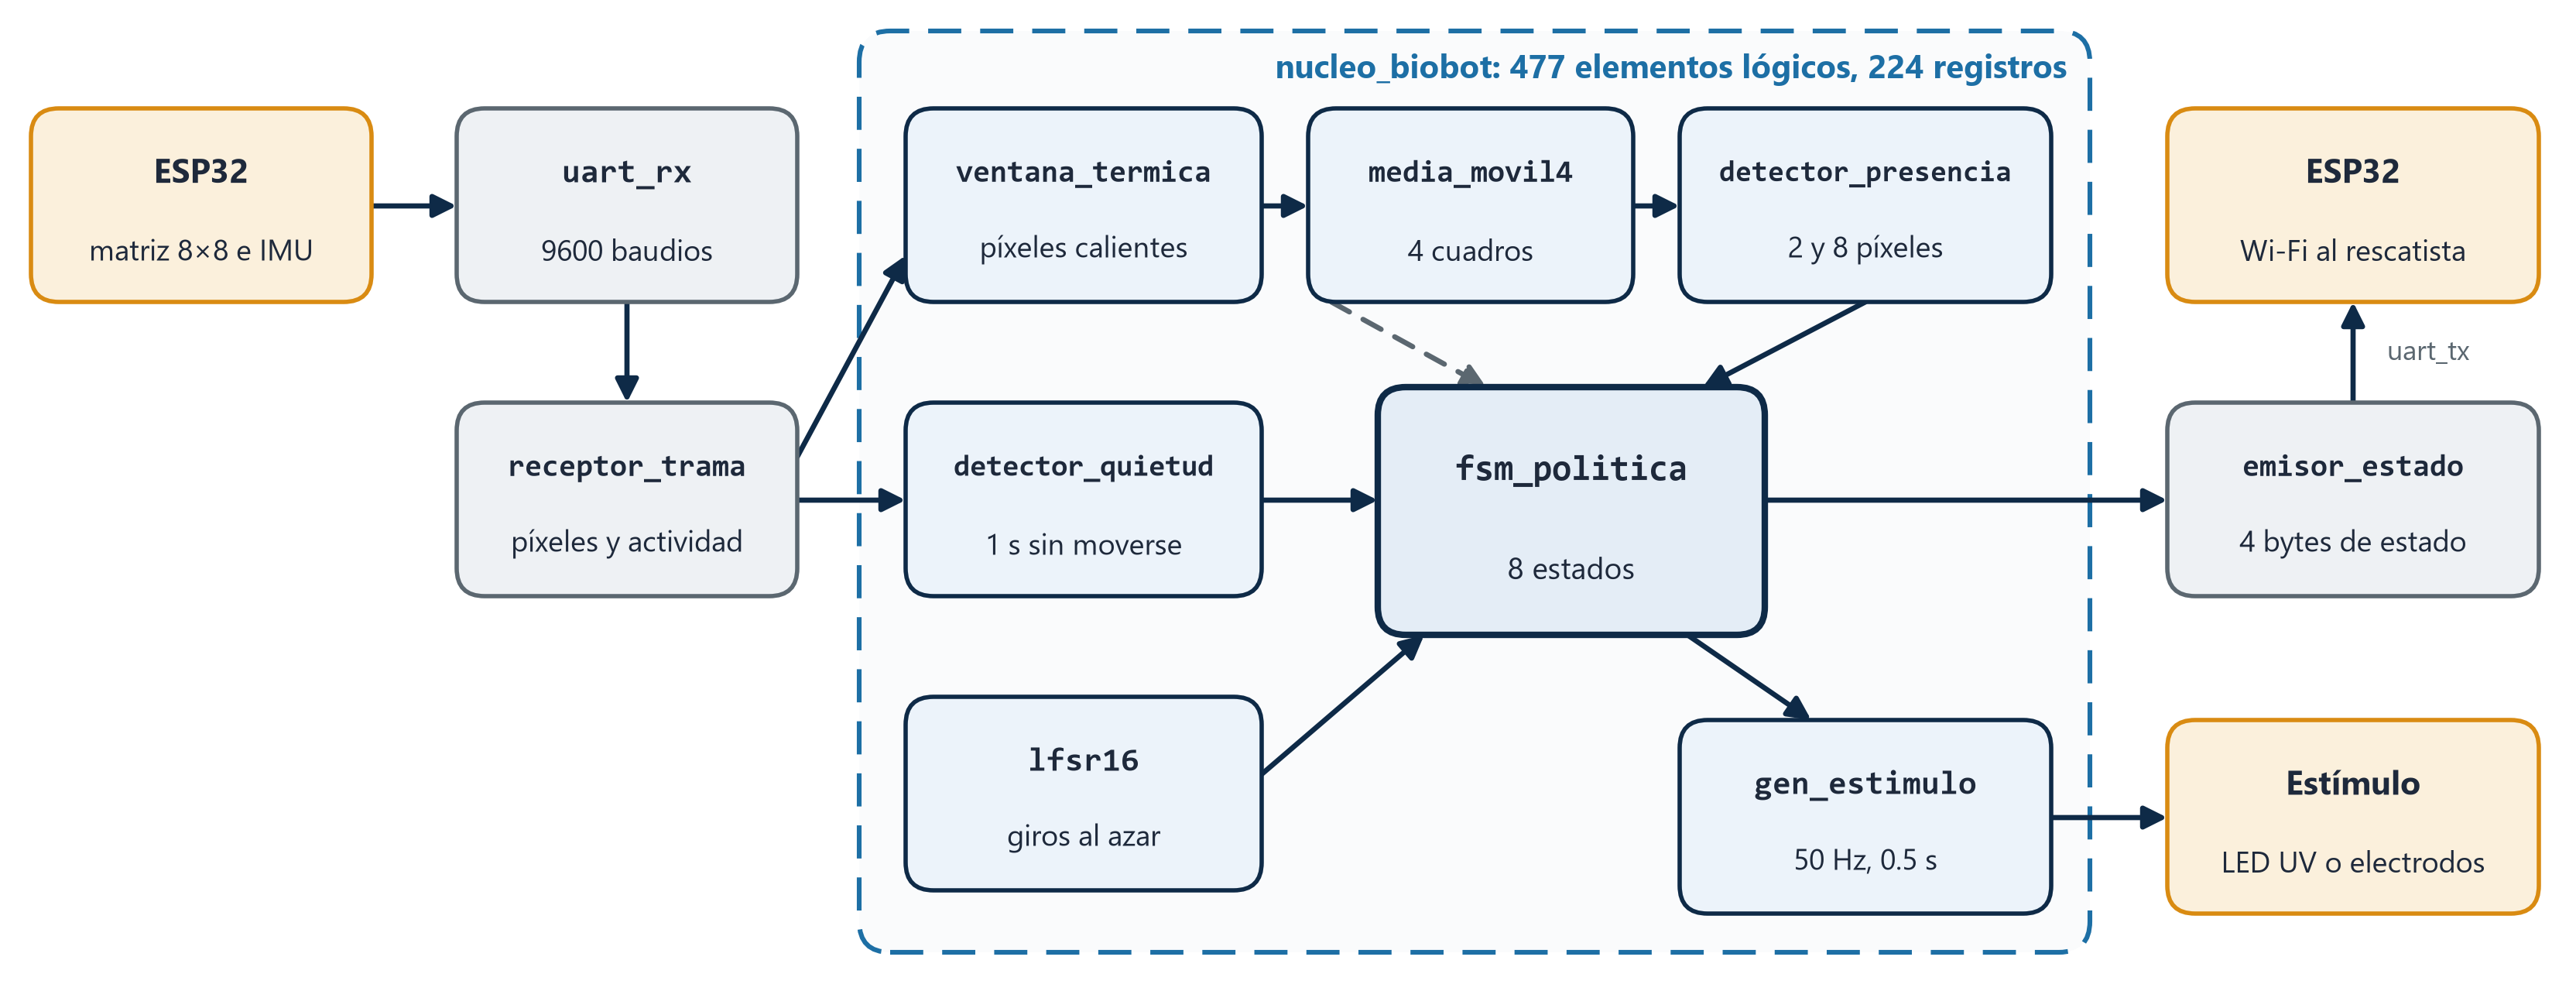
\includegraphics[width=\textwidth]{figs/nucleo_digital.png}
\caption{Módulos Verilog del núcleo y del enlace serie del prototipo.}
\label{fig:nucleo}
\end{figure}

\modulo{ventana\_termica}{hdl/ventana\_termica.v}{160 EL, 61 R}
Recibe la matriz píxel por píxel, un byte de 0.25~\textdegree C por cuenta con un pulso \sig{px\_valido}. Dos
comparadores revisan la ventana de piel ($T_{\min}\le T\le T_{\max}$, por omisión 112 y 152 cuentas, o sea 28 y
38~\textdegree C) y un tercero exige superar el fondo en 8 cuentas (2~\textdegree C); si los tres se cumplen, el
píxel es caliente. Tres contadores llevan el total, los de las columnas 0 a 2 y los de las columnas 5 a 7, y un
acumulador de 14 bits suma las temperaturas. Con \sig{px\_ultimo} cierra el cuadro: publica el conteo, el lado
que domina (01 izquierda, 10 derecha, 00 centro) y la media, que se obtiene con un corrimiento de 6 bits y sirve
de fondo para el cuadro siguiente. Los valores se calculan con el píxel actual ya sumado, así que todo cierra en
el mismo ciclo. El fondo arranca en 255: en el primer cuadro nada puede ser caliente. El pulso \sig{cuadro} es el
\sig{tick} con el que avanzan los demás módulos (figura~\ref{fig:dventana}).

\begin{figure}[!htb]
\centering
\begin{subfigure}{\textwidth}
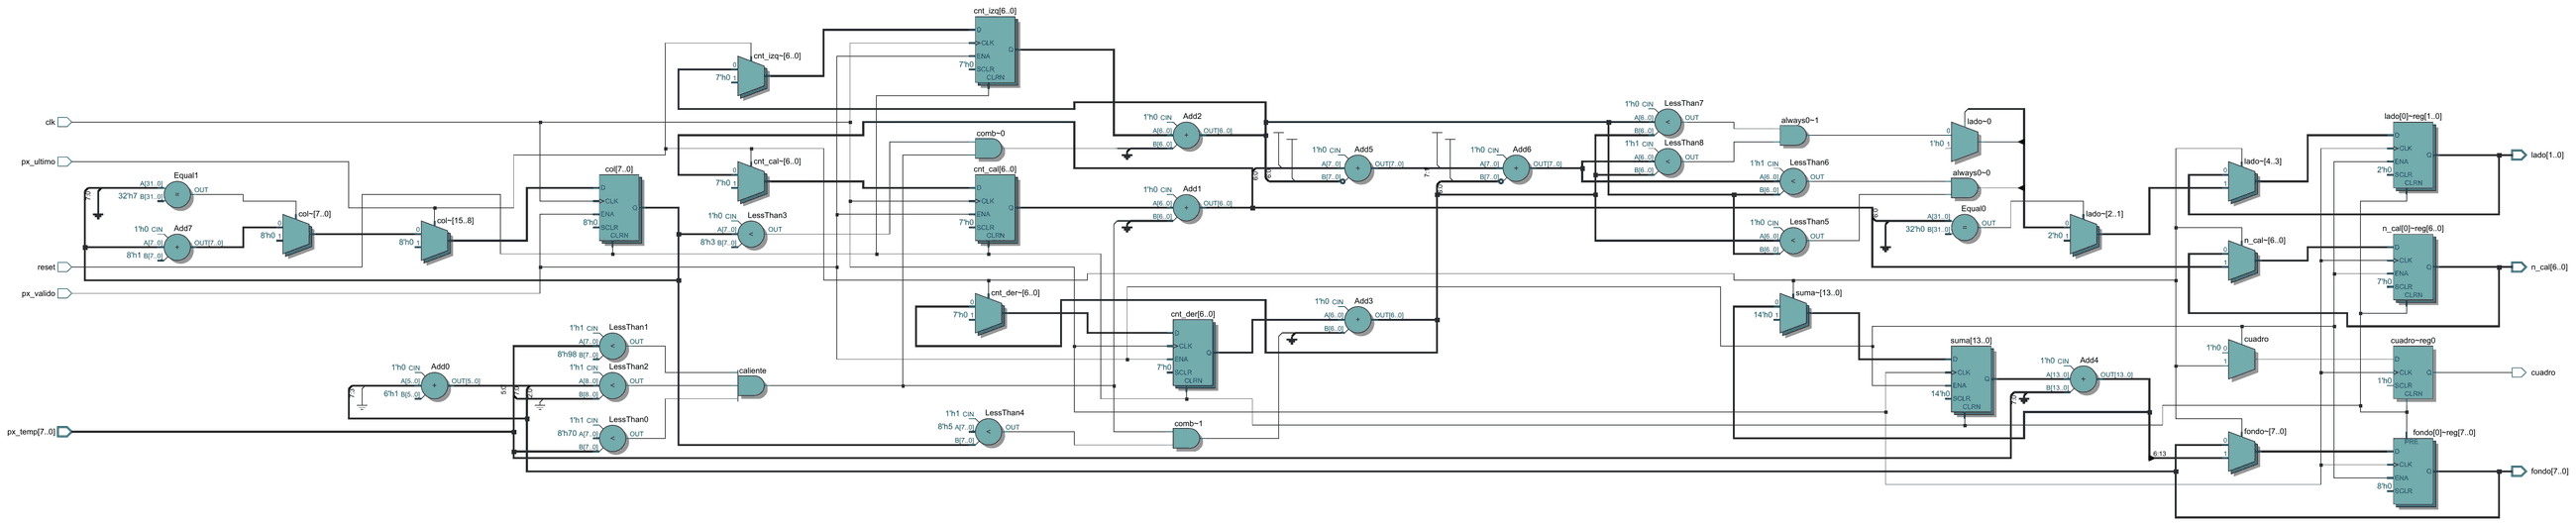
\includegraphics[width=\linewidth]{figs/rtl/rtl_ventana_termica.png}
\caption{El módulo completo.}
\end{subfigure}

\medskip
\begin{subfigure}{0.46\textwidth}
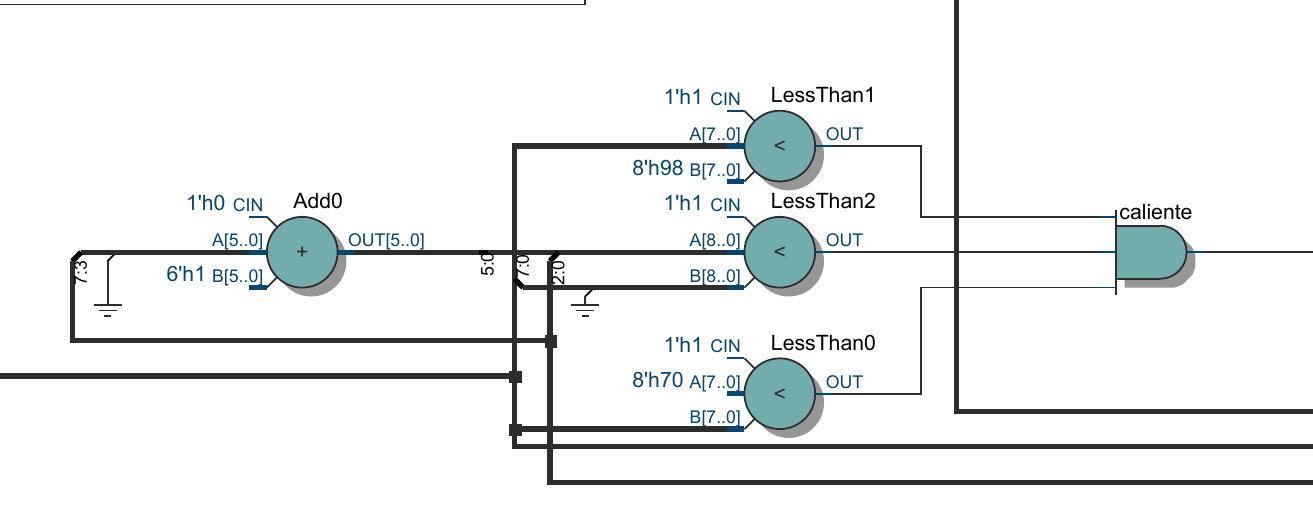
\includegraphics[width=\linewidth]{figs/rtl/zoom_ventana_termica.png}
\caption{Acercamiento: los tres comparadores (\sig{8'h70} = 28~\textdegree C, \sig{8'h98} = 38~\textdegree C y el fondo más 8) y la compuerta \sig{caliente}.}
\end{subfigure}
\caption{\sig{ventana\_termica} en el RTL Viewer de Quartus.}
\label{fig:dventana}
\end{figure}

\modulo{media\_movil4}{hdl/detectores.v}{40 EL, 28 R}
Filtro FIR de cuatro coeficientes iguales (sección~\ref{sec:fir}). Guarda los últimos cuatro conteos en un
registro de corrimiento, los suma con dos bits extra para no desbordar y divide entre cuatro quitando los dos
bits bajos. Quita el vaivén que mete el insecto al caminar.

\modulo{detector\_presencia}{hdl/detectores.v}{9 EL, 4 R}
Compara el conteo filtrado con dos umbrales: \sig{pre} vale 1 con 2 píxeles o más (conviene acercarse) y
\sig{sobre}, con 8 o más. Un contador de 4 bits, que se satura en 15, cuenta los cuadros seguidos con
\sig{sobre} y vuelve a cero en cuanto falta uno; al llegar a cuatro levanta \sig{confirmado}. Así un reflejo de un
solo cuadro no dispara la alerta.

\modulo{detector\_quietud}{hdl/detectores.v}{10 EL, 4 R}
Recibe la «actividad» de la IMU (0 a 255). Si se queda por debajo de 8 durante diez cuadros seguidos, un segundo,
declara quieto al insecto; una sola lectura por arriba baja la salida de inmediato.

\modulo{lfsr16}{hdl/detectores.v}{16 EL, 16 R}
Registro de corrimiento con realimentación, $x^{16}+x^{14}+x^{13}+x^{11}+1$, de periodo 65\,535 y semilla
\sig{0xACE1}. Avanza un paso por cuadro. La política gira al azar cuando sus nueve bits bajos son cero, es decir
una vez cada 512 cuadros (51.2~s) en promedio, y el bit 9 decide el lado.

\modulo{fsm\_politica}{hdl/fsm\_politica.v}{181 EL, 64 R}
Es el control. Un bloque combinacional calcula el estado siguiente y si este cuadro sale un estímulo; un bloque
secuencial lo registra y actualiza los temporizadores, todos en décimas de segundo:
\begin{itemize}
  \item \textbf{REPOSO} espera la orden de arranque. \textbf{EXPLORAR} deja caminar y vigila, en este orden, la
        mancha de calor, el presupuesto, la quietud y el azar.
  \item \textbf{REACTIVAR}: tras 15~s quieto manda un pulso de avance y observa 3~s. Si arranca, la espera vuelve a
        15~s; si no, se duplica hasta 120~s. \textbf{REORIENTAR} gira a un lado al azar y regresa a explorar.
  \item \textbf{ACERCAR}: con \sig{pre} gira hacia el lado de la mancha, o avanza si está quieto; si la pierde 5~s,
        vuelve a explorar. \textbf{CONFIRMAR} deja de estimular y espera \sig{confirmado}. \textbf{ALERTAR} es final y
        emite una baliza cada 5~s. \textbf{DESCANSO} espera a que baje el presupuesto.
\end{itemize}
Entre estímulos pasan al menos 10~s. El presupuesto es una cuenta Q8.8: cada estímulo suma 256 (1.0) y cada 23
cuadros pierde $1/256$ de su valor, al menos una cuenta, lo que da una constante de unos 590~s, cercana a la
recuperación del insecto. Con 12.0 acumulados se deja de estimular. Así se acota la habituación y la carga sobre
el animal sin medir su respuesta.

\modulo{gen\_estimulo}{hdl/gen\_estimulo.v}{64 EL, 47 R}
Con cada \sig{disparo} saca 25 periodos de una onda cuadrada de 50~Hz (0.5~s) por el canal pedido: avance,
izquierda o derecha. Un contador mide el medio periodo (500\,000 ciclos a 50~MHz) y un bit alterna las mitades.
Cada canal tiene dos salidas en contrafase, \sig{fase\_a} y \sig{fase\_b}, que en un par de electrodos dan una
onda bifásica sin componente continua; para la luz ultravioleta basta \sig{led\_on}. Mientras hay un tren en
curso ignora otros disparos, y todas las salidas son registros para no tener transitorios.

\modulo{nucleo\_biobot}{hdl/nucleo\_biobot.v}{477 EL, 224 R}
Conecta los siete módulos. No depende de la tarjeta: recibe píxeles ya separados y la actividad, y entrega las
fases, el estado, la alerta, la baliza y la telemetría. Es el mismo archivo en la demostración, en la red de tres
tarjetas (donde la ventana se ajusta a 35--38~\textdegree C por parámetros) y en el layout. La
figura~\ref{fig:rtlnucleo} es lo que Quartus entiende de él.

\begin{figure}[!htb]
\centering
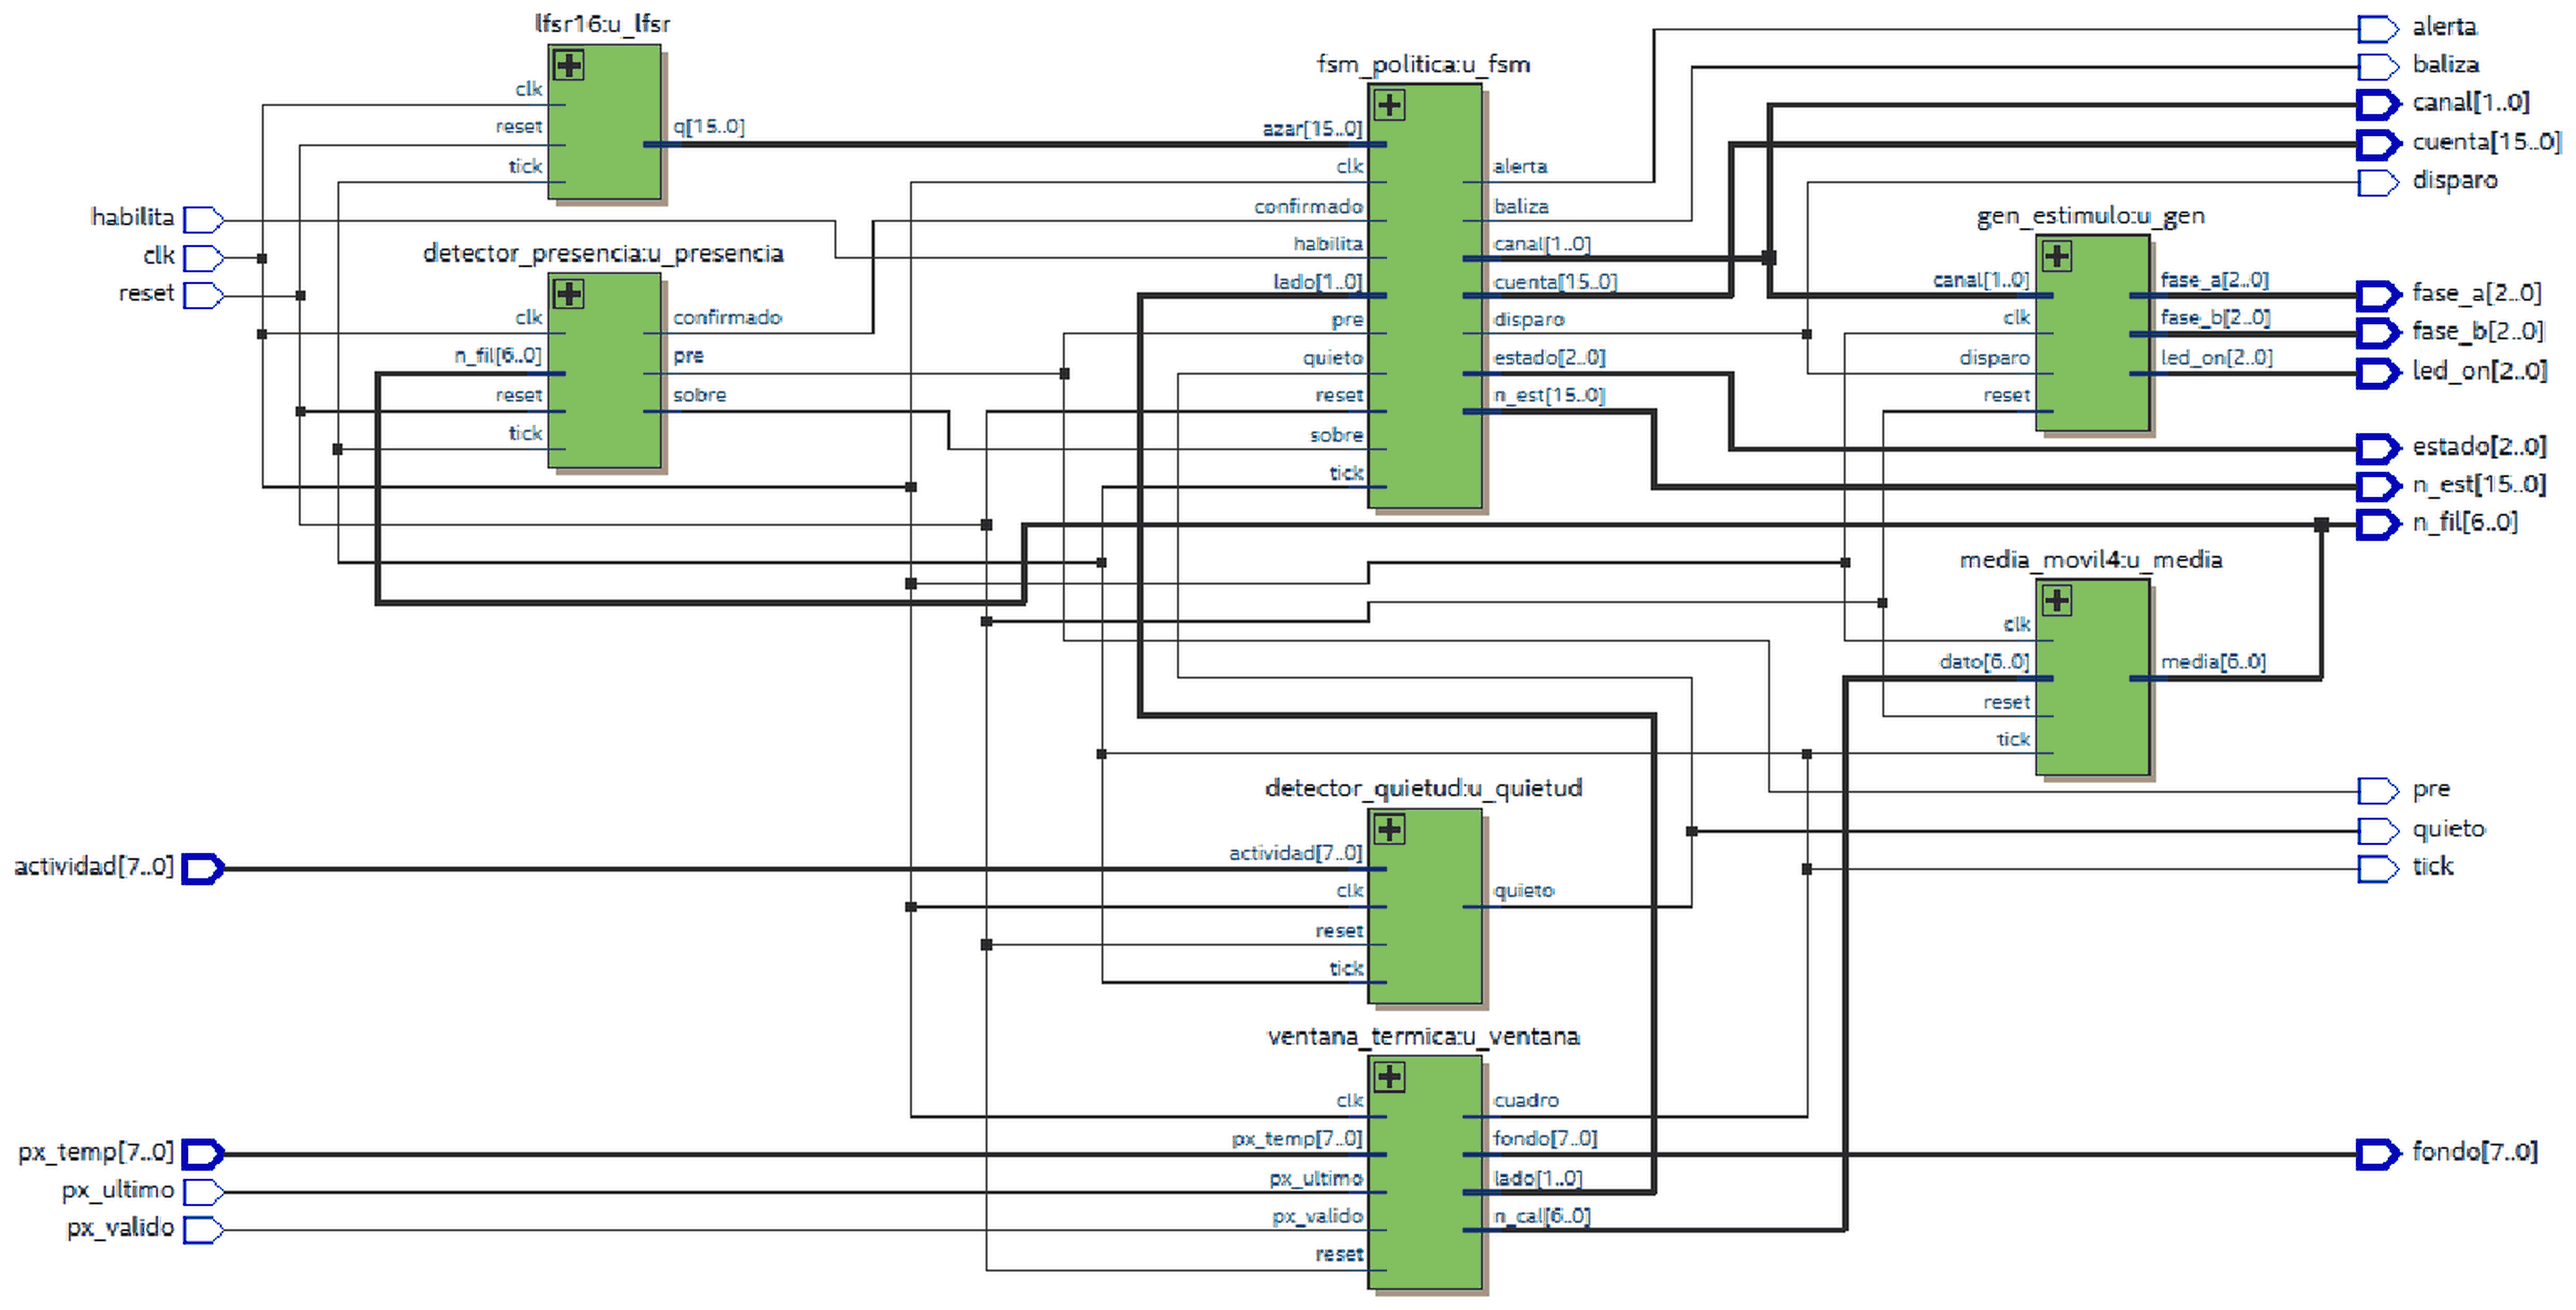
\includegraphics[width=0.94\textwidth]{figs/rtl/rtl_nucleo.png}
\caption{\sig{nucleo\_biobot} en el RTL Viewer de Quartus: los siete módulos y sus conexiones.}
\label{fig:rtlnucleo}
\end{figure}

\subsubsection{Enlace serie del prototipo}

\modulo{uart\_rx}{hdl/uart\_rx.v}{63 EL, 40 R}
Receptor 8N1 de la práctica~4. Dos flip-flops sincronizan la línea; al ver el flanco de bajada espera medio bit y
confirma que el bit de inicio sigue en 0 (si no, fue ruido y lo descarta). Desde ahí cuenta bits completos
(5\,208 ciclos a 9\,600 baudios o 434 a 115\,200) y muestrea cada dato en su centro, empezando por el menos
significativo. En el centro del bit de paro entrega el byte con un pulso \sig{data\_valid}
(figura~\ref{fig:duart}).

\begin{figure}[!htb]
\centering
\begin{tikzpicture}[x=1.22cm,y=0.75cm,every node/.style={font=\scriptsize}]
\draw[thick,Primary] (-0.8,1) -- (0,1) -- (0,0) -- (1,0);
\foreach \i in {1,...,8} {\draw[thick,Primary] (\i,0) rectangle (\i+1,1); \node at (\i+0.5,1.35) {$d_{\the\numexpr\i-1\relax}$};}
\draw[thick,Primary] (9,0) -- (9,1) -- (10.6,1);
\node at (0.5,1.35) {inicio}; \node at (9.6,1.35) {paro}; \node at (-0.55,1.35) {reposo};
\foreach \i in {0,...,9} {\draw[Accent,very thick,-{Stealth[length=1.6mm]}] (\i+0.5,-0.85) -- (\i+0.5,-0.1);}
\draw[<->,Secondary] (0,-0.35) -- (0.5,-0.35); \node[Secondary] at (0.1,-0.75) {$\tfrac12$ bit};
\draw[<->,Secondary] (2.5,-0.35) -- (3.5,-0.35); \node[Secondary] at (3,-0.75) {1 bit};
\node[Accent] at (5,-1.2) {muestreo en el centro de cada bit; en el de paro sale \sig{data\_valid}};
\end{tikzpicture}
\caption{Instantes en que \sig{uart\_rx} lee la línea.}
\label{fig:duart}
\end{figure}

\modulo{uart\_tx}{hdl/uart\_tx.v}{43 EL, 31 R}
Con \sig{tx\_start} carga un registro de diez bits, \sig{\{1, dato, 0\}}, y lo recorre a la derecha un bit por
periodo. Mientras transmite, \sig{busy} vale 1 y no acepta otra petición.

\modulo{receptor\_trama}{hdl/enlace\_serie.v}{86 EL, 58 R}
Arma un cuadro con los bytes que llegan: \sig{0xA5}, actividad y 64 píxeles. La actividad va primero para que esté
estable cuando el último píxel cierra el cuadro. Si pasan 5~ms sin bytes, abandona la trama y vuelve a buscar la
cabecera.

\modulo{emisor\_estado}{hdl/enlace\_serie.v}{31 EL, 16 R}
Después de cada cuadro contesta cuatro bytes: \sig{0x5A}; alerta, estado, si hubo estímulo, canal y quietud;
\sig{pre} y conteo filtrado; y la parte entera del presupuesto. Espera tres ciclos tras el \sig{tick} para leer el
estado ya actualizado y guarda el disparo en un bit para no perderlo entre reportes.

\subsubsection{Verificación contra un modelo de referencia}

Antes de escribir el Verilog se programó en Python un modelo que hace las mismas cuentas con enteros, registro por
registro. Genera los cuadros de prueba y la respuesta esperada, y los bancos comparan cuadro por cuadro
(tabla~\ref{tab:bancos}). El prototipo completo ocupa 722~EL y 372~R, con $f_{\max}=72.08$~MHz.

\begin{table}[!htb]
\centering\footnotesize
\caption{Resultados de simulación del núcleo con Icarus Verilog 12.}
\label{tab:bancos}
\rowcolors{2}{SoftGray}{white}
\begin{tabularx}{\textwidth}{@{}>{\ttfamily\raggedright\arraybackslash}p{2.7cm} >{\raggedright\arraybackslash}X >{\raggedright\arraybackslash}p{5.0cm}@{}}
\toprule
\rowcolor{TableHead} \normalfont\textbf{Banco} & \textbf{Qué prueba} & \textbf{Resultado} \\
\midrule
tb\_nucleo & Pausas, insecto que no responde, acercamiento, ambiente a 30 y 37.5~\textdegree C, objeto a 47.5~\textdegree C y 3\,000 cuadros al azar & 11\,424 de 11\,424 cuadros coinciden; se visitan los ocho estados \\
tb\_gen\_estimulo & Periodo, ciclo, duración, fases y disparo a medio tren & 3 de 3 trenes: 25 periodos de 20.000~ms \\
tb\_top & Sistema completo por UART hasta la detección & 500 de 500 respuestas coinciden \\
tb\_demo & Núcleo e insecto de prueba en el mismo chip & 4 de 4: alerta solo con persona, cuadro 558 \\
tb\_dos\_tarjetas & Dos tarjetas unidas solo por UART & 2 de 2: alerta en el cuadro 557 \\
\bottomrule
\end{tabularx}
\end{table}

\subsection{La red de tres FPGA}
\label{sec:red}

Una mochila que detecta sola no le dice al rescatista dónde cavar, y su radio no atraviesa el
concreto (sección~\ref{sec:deteccion}). La red resuelve las dos cosas con lo que ya hay en el
escombro: otra mochila. Dos mochilas que ven a la misma persona desde lugares distintos
bastan para ubicarla, y la que quedó cerca de la entrada retransmite el aviso de la que quedó
lejos. La demostración usa tres DE10-Lite (figura~\ref{fig:tresfpga}): dos hacen de mochilas
de dos insectos, A y B, y la tercera es el receptor del operador, en la entrada del derrumbe.

\begin{figure}[H]
\centering
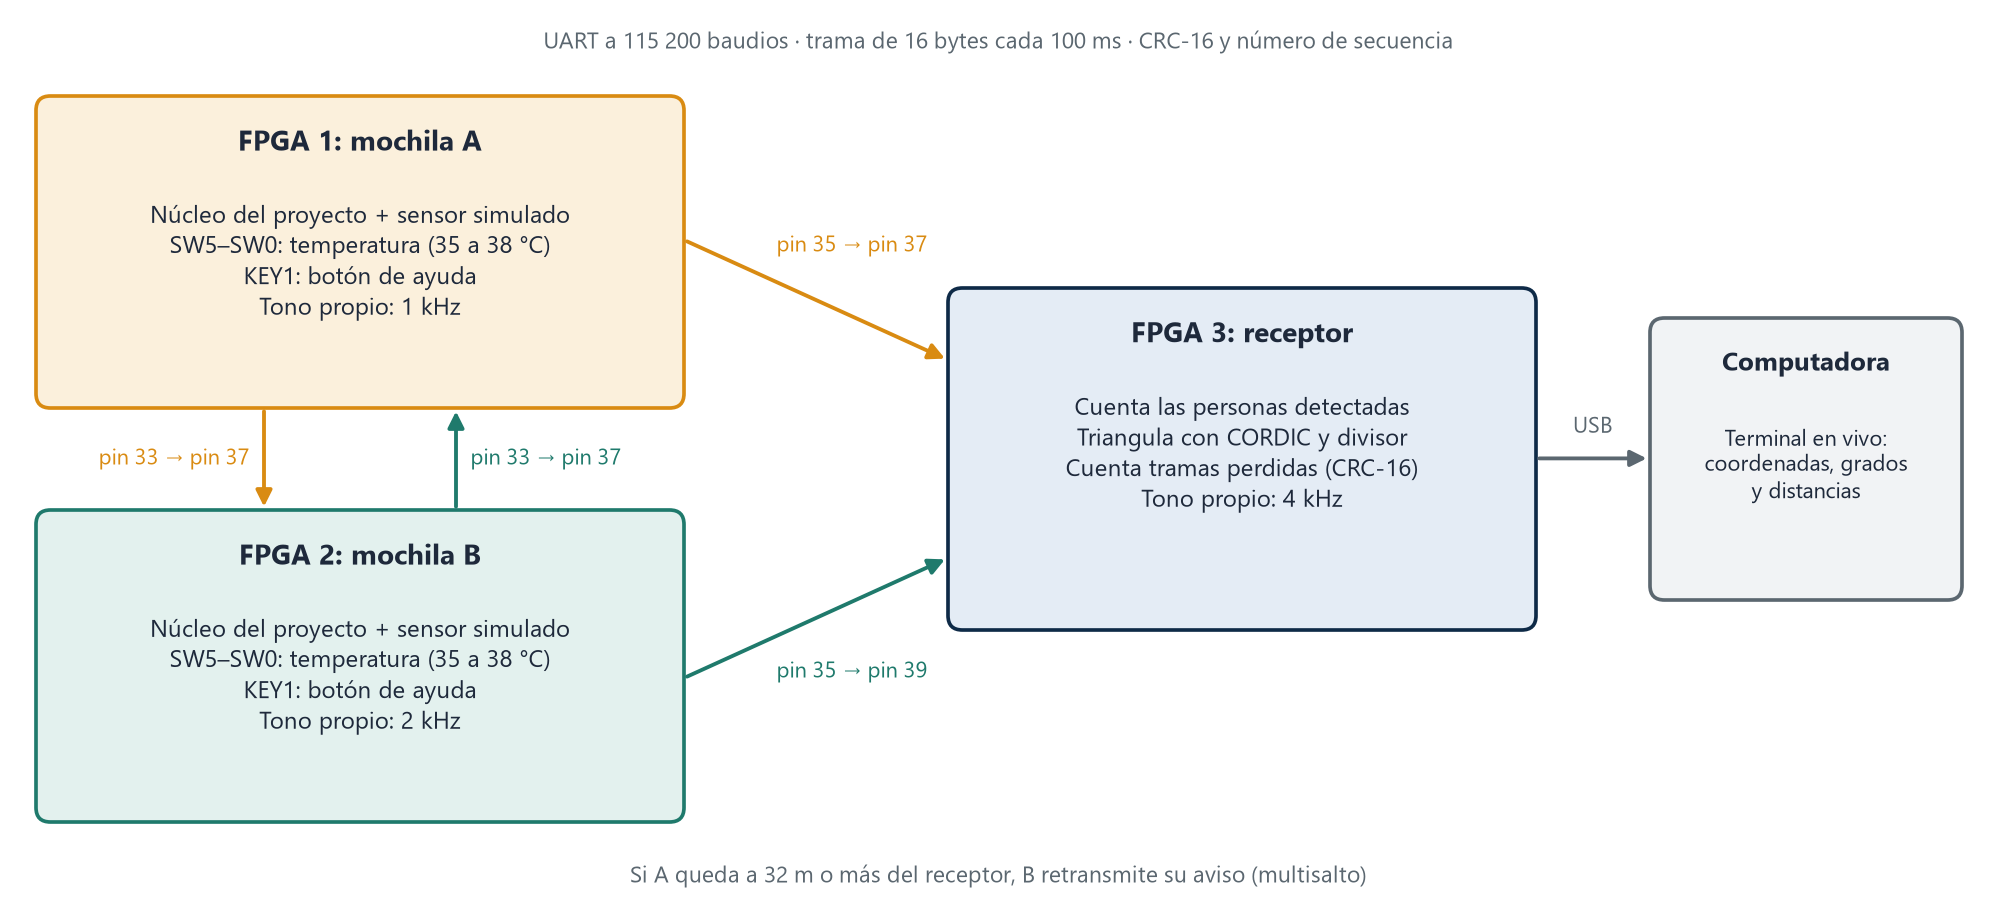
\includegraphics[width=\textwidth]{figs/red_tres_fpga.png}
\caption{Las tres tarjetas, sus enlaces por UART y la computadora del operador.}
\label{fig:tresfpga}
\end{figure}

\subsubsection{Qué hace cada nodo}

\begin{itemize}
  \item \textbf{Cada mochila} corre el núcleo de la sección~\ref{sec:nucleo}, sin cambiarle nada, sobre
        un sensor térmico simulado: los interruptores SW5--SW0 fijan, en grados y en binario, la
        temperatura que lee la matriz. Detecta a una persona de dos formas redundantes: por
        temperatura, entre 35 y 38~\textdegree C, y por el botón de ayuda que va sobre el insecto.
        Mide en qué dirección ve el calor, emite un tono propio, transmite su estado diez veces por
        segundo y retransmite una vez las tramas de la otra mochila.
  \item \textbf{El receptor} junta lo que llega, cuenta las personas detectadas, cruza los rumbos de
        las dos mochilas para estimar dónde está la persona y deja todo en registros que la
        computadora lee.
  \item \textbf{La computadora} muestra esos registros en una terminal y manda órdenes de prueba.
        No hace ninguna cuenta del sistema (tabla~\ref{tab:reparto}).
\end{itemize}

Los parámetros de la demostración son parámetros de los módulos, con nombre
(tabla~\ref{tab:parametrosred}).

\begin{table}[H]
\centering\footnotesize
\caption{Parámetros de la demostración y dónde están en el código.}
\label{tab:parametrosred}
\rowcolors{2}{SoftGray}{white}
\begin{tabularx}{\textwidth}{@{}>{\bfseries\raggedright\arraybackslash}p{3.6cm} >{\raggedright\arraybackslash}X >{\raggedright\arraybackslash}p{4.3cm}@{}}
\toprule
\rowcolor{TableHead} Parámetro & Valor & En el código \\
\midrule
Ventana de temperatura de una persona & 35 a 38~\textdegree C, las dos incluidas & \sig{T\_PERSONA\_MIN}, \sig{T\_PERSONA\_MAX} \\
Sensor térmico simulado & SW5--SW0: grados en binario, de 0 a 63 & \sig{sw[5:0]} de \sig{tri\_mochila} \\
Segunda detección & KEY1 sostenido 0.1~s; queda marcado hasta el reset & \sig{T\_PULSA\_MS} \\
Conteo de personas & 0, 1 o 2, igual en las tres tarjetas y en la terminal; baja si la temperatura sale de la ventana & \sig{cuenta\_pd}, \sig{REARMA} \\
Alcance del radio y de los tonos & Menos de 32~m: a 31~m se oye; a 32~m o más, no & \sig{ALCANCE\_M} \\
Escala de distancias & 10 bits, de 0 a 64~m: 6.25~cm por cuenta. Cinco metros son 80 cuentas, el 7.8~\% de la escala & \sig{tri\_distancia} \\
Tonos & A 1~kHz, B 2~kHz y receptor 4~kHz; umbral de potencia de 4\,000 & \sig{tri\_tonos}, \sig{UMBRAL} \\
Enlace & UART 8N1 a 115\,200 baudios; trama de 16 bytes cada 100~ms & \sig{BAUD\_RATE}, \sig{tri\_tx\_n}, \sig{tri\_rx\_n} \\
\bottomrule
\end{tabularx}
\end{table}

\subsubsection{Lo que se ve en cada tarjeta}

\begin{table}[H]
\centering\footnotesize
\caption{Displays y LED de la red. Un guion en HEX1 o HEX0 quiere decir que no se oye a ese nodo.}
\label{tab:displays}
\rowcolors{2}{SoftGray}{white}
\begin{tabularx}{0.92\textwidth}{@{}>{\bfseries\raggedright\arraybackslash}p{2.2cm} >{\raggedright\arraybackslash}X >{\raggedright\arraybackslash}X@{}}
\toprule
\rowcolor{TableHead} Indicador & En una mochila & En el receptor \\
\midrule
HEX5 & Quién es: \sig{A} o \sig{b} & \sig{r} \\
HEX4--HEX3 & \sig{Pd}, personas detectadas & \sig{Pd} \\
HEX2 & Cuántas: 0, 1 o 2 & Lo mismo \\
HEX1 & La letra de la otra mochila, si oye su tono & \sig{A}, si oye el tono de A \\
HEX0 & \sig{r}, si oye el tono del receptor & \sig{b}, si oye el tono de B \\
LEDR9--5 & Metros a la otra mochila, en binario & Metros a la mochila A \\
LEDR4--0 & Metros al receptor & Metros a la mochila B \\
\bottomrule
\end{tabularx}
\end{table}

Con cinco LED se cuentan hasta 31~m, que es justo el alcance. Los metros van sin redondear
(31.9~m marca 31), y un nodo que se oye marca al menos 1 aunque esté a menos de un metro: así,
los cinco LED apagados quieren decir siempre «no lo oigo».

\subsubsection{Mapa, escala y alcance}

Las posiciones van en 10 bits sobre un mapa de 0 a 64~m, de modo que una cuenta vale 6.25~cm.
El receptor está en $(0,0)$ y la persona en $(25.50,\,19.25)$~m, a 31.95~m: justo en el borde
del alcance. Por eso, de dos mochilas que están junto a la persona, una puede quedar dentro
del alcance y la otra fuera, y entonces la primera hace de puente (figura~\ref{fig:mapared}).

\begin{figure}[H]
\centering
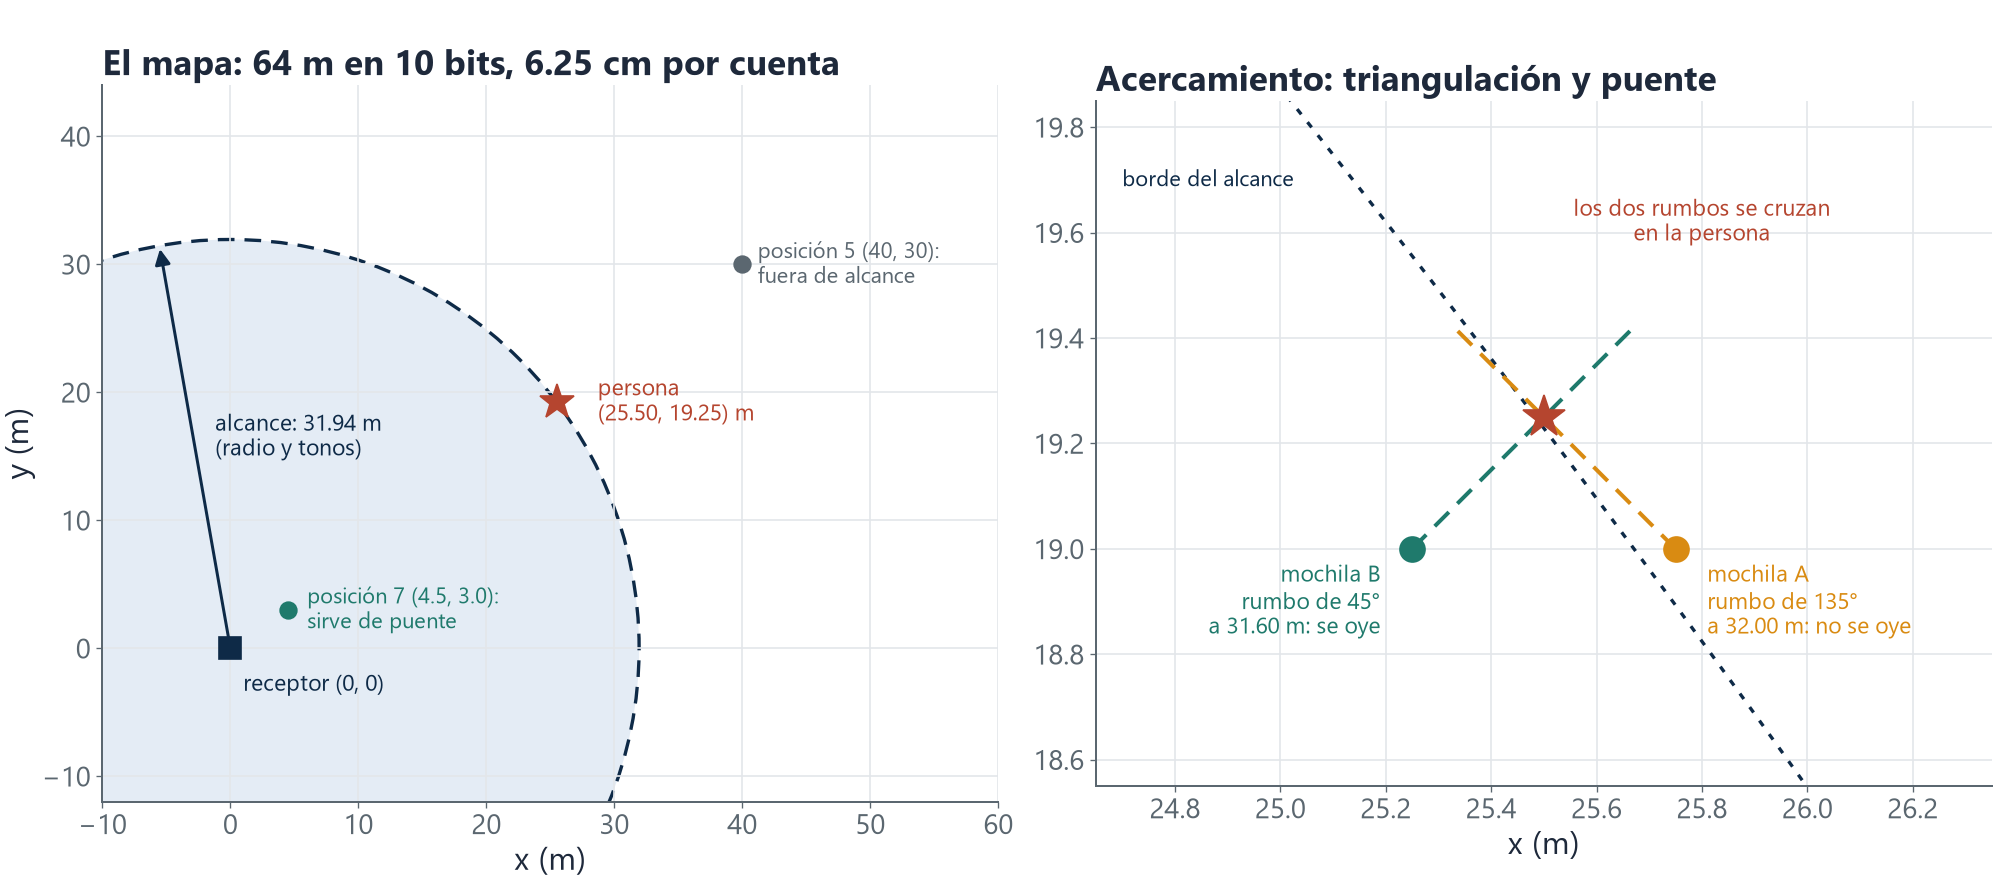
\includegraphics[width=\textwidth]{figs/red_mapa.png}
\caption{El mapa de 64~m con el alcance de 32~m, y el acercamiento donde se cruzan los dos rumbos.}
\label{fig:mapared}
\end{figure}

La distancia entre dos nodos se calcula exacta, con una raíz cuadrada entera
(sección~\ref{sec:raiz}), y la regla del alcance usa la misma suma de cuadrados:
\begin{equation}
d=\left\lfloor\sqrt{\Delta x^2+\Delta y^2}\,\right\rfloor\ \text{cuentas},\qquad
\text{se oye si}\quad \Delta x^2+\Delta y^2<(16\times32)^2 .
\label{eq:alcance}
\end{equation}
Como las dos salen del mismo número, no pueden contradecirse: un nodo se oye exactamente
cuando su distancia marca menos de 32.00~m.

\subsubsection{Protocolo de enlace}

El enlace es UART 8N1 a 115\,200 baudios, el de la práctica~4, con una trama propia de 16 bytes
que cada mochila transmite cada 100~ms (figura~\ref{fig:trama}).

\begin{figure}[H]
\centering
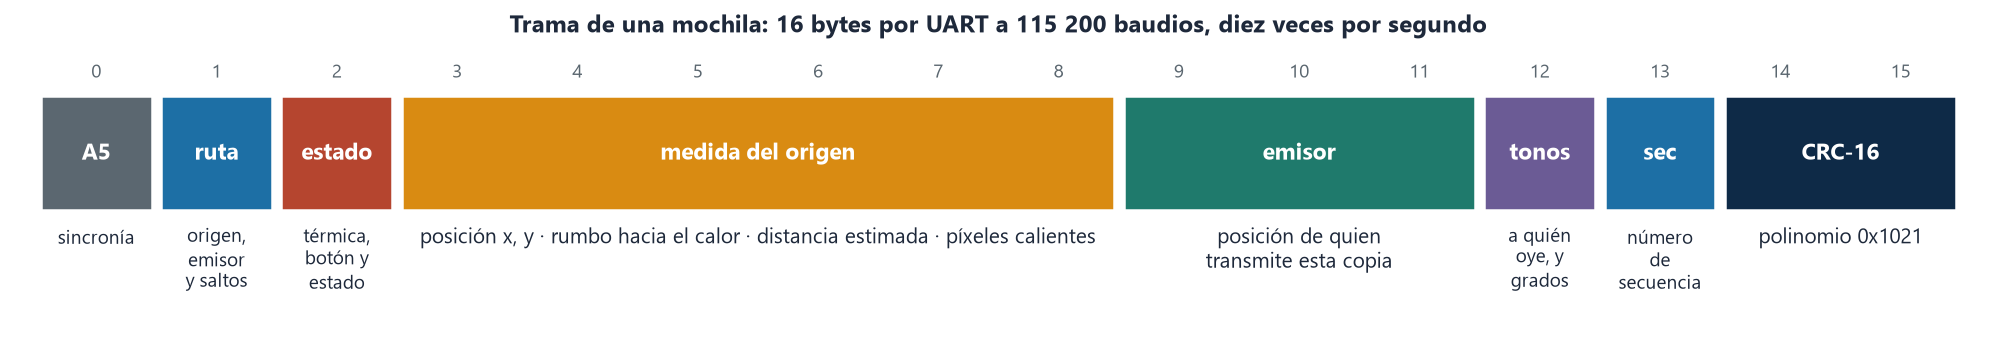
\includegraphics[width=\textwidth]{figs/red_trama.png}
\caption{Los 16 bytes de la trama de una mochila.}
\label{fig:trama}
\end{figure}

El byte de ruta distingue al \emph{origen}, la mochila que midió, del \emph{emisor}, la que
transmite esta copia. Quien recibe aplica cinco reglas:
\begin{itemize}
  \item Descarta la trama si el CRC-16 no coincide o si se interrumpe más de 2~ms. El CRC usa el
        polinomio \sig{0x1021} con valor inicial \sig{0xFFFF} sobre los bytes 1 a 13; un código
        cíclico de 16 bits detecta toda ráfaga de errores de 16 bits o menos~\cite{peterson1961}.
  \item Solo la acepta si el emisor está a menos de 32~m: así se simula el alcance del radio.
  \item Una mochila reenvía una sola vez las tramas de la otra, con el contador de saltos
        incrementado. Es lo que permite el puente.
  \item Con el número de secuencia, el receptor cuenta las tramas perdidas y reconoce la que le
        llega repetida por dos caminos.
  \item Si en un segundo no llega nada de una mochila, la da por perdida.
\end{itemize}

\subsubsection{Reconocer a los vecinos por tonos}

La radio dice qué mide cada mochila, pero no quién le queda cerca. Para eso cada nodo emite todo
el tiempo un tono distinto (A 1~kHz, B 2~kHz y el receptor 4~kHz) y escucha los otros dos: con
saber a quién oye, sabe quién está a su alcance, sin conocer su posición. Cada nodo muestrea su
micrófono a 16~kHz y, cada 64 muestras (4~ms), tres filtros de Goertzel~\cite{goertzel1958}
miden la potencia en las tres frecuencias (sección~\ref{sec:goertzel}). Un tono se da por oído
si su potencia pasa del umbral en dos bloques seguidos, y por perdido si queda debajo en dos.

En la demostración no hay bocinas ni micrófonos. El canal acústico va simulado dentro de la
FPGA: la señal del micrófono es la suma de las ondas cuadradas de los nodos que están a menos
de 32~m, más ruido, y los filtros trabajan sobre esa señal como lo harían sobre la real. Para
probarlo con hardware bastan dos cambios, y ninguno toca los filtros: el tono propio ya sale
por el pin~1 del conector JP1, listo para un zumbador, y la suma simulada se sustituye por las
muestras de un micrófono con su convertidor.

\subsubsection{Rumbo y triangulación}

Cada mochila mide el rumbo hacia el calor: el centroide de las columnas calientes de la matriz,
que da el ángulo respecto al frente del insecto, más el rumbo del insecto. El receptor cruza las
dos rectas que salen de A y de B con esos rumbos:
\begin{equation}
P=A+t\,\hat u_A,\qquad t=\frac{(B-A)\times\hat u_B}{\hat u_A\times\hat u_B},
\qquad \hat u=(\cos\theta,\ \sin\theta).
\label{eq:triangula}
\end{equation}
Los cosenos y senos salen de un CORDIC en rotación y el cociente de un divisor con restauración
(sección~\ref{sec:cordic}); no hay tablas de seno ni funciones de biblioteca. El módulo distingue
tres casos en los que el cruce no sirve y lo indica: rumbos casi paralelos (menos de
10\textdegree{} entre sí), rectas que se cruzan detrás de una mochila y cruce a más de 3~m. En
esos casos, o si solo una mochila detecta, el receptor usa la aproximación de cada mochila por
separado: su posición más la distancia que estima por el tamaño de la mancha.

\textbf{El sensor simulado no altera el núcleo.} El módulo \sig{tri\_escena} conoce la posición
de la persona; con la posición y el rumbo del insecto calcula, con un CORDIC en vectorización,
en qué columna de la matriz caería la mancha, y entrega los 64 píxeles con la temperatura de
los interruptores sobre un fondo de 22~\textdegree C. El núcleo recibe esos píxeles como los
recibiría del sensor.

\subsubsection{Reparto entre la FPGA y la computadora}

\begin{table}[H]
\centering\footnotesize
\caption{Dónde corre cada función del sistema.}
\label{tab:reparto}
\rowcolors{2}{SoftGray}{white}
\begin{tabularx}{0.9\textwidth}{@{}>{\raggedright\arraybackslash}X >{\raggedright\arraybackslash}p{4.2cm}@{}}
\toprule
\rowcolor{TableHead} \textbf{Función} & \textbf{Dónde corre} \\
\midrule
Detección térmica, filtrado, decisión y estímulo & FPGA (mochila) \\
Rumbo hacia el calor & FPGA (mochila) \\
Tramas, CRC-16, número de secuencia, alcance y puente & FPGA (las tres) \\
Generación y detección de tonos & FPGA (las tres) \\
Distancias exactas entre nodos & FPGA (las tres) \\
Conteo de personas y triangulación & FPGA (receptor) \\
Displays y LED & FPGA (las tres) \\
Mostrar los datos y mandar órdenes de prueba & Computadora \\
\bottomrule
\end{tabularx}
\end{table}

La computadora lee por el cable USB-Blaster los registros del receptor, con una sonda de
Quartus (\emph{In-System Sources and Probes}~\cite{intelissp}), los convierte a metros y grados
y los escribe en pantalla; no hace falta ningún adaptador serie. Por la misma sonda puede
fijar la posición y la temperatura de cada mochila, que es como se prueban el alcance y el
puente sin mover cables. Si la computadora se desconecta, las tres tarjetas siguen funcionando
igual: los displays y los LED no dependen de ella.

\subsection{Módulos numéricos en punto fijo (práctica 5)}
\label{sec:numerico}

La red necesita ángulos, cosenos, potencias de un tono y distancias, y en la FPGA no hay punto flotante. La
tabla~\ref{tab:formatos} resume los formatos; cada bloque se comparó contra el valor exacto.

\begin{table}[!htb]
\centering\footnotesize
\caption{Formatos de punto fijo del proyecto.}
\label{tab:formatos}
\rowcolors{2}{SoftGray}{white}
\begin{tabularx}{\textwidth}{@{}>{\bfseries\raggedright\arraybackslash}p{3.2cm} >{\raggedright\arraybackslash}p{4.4cm} >{\raggedright\arraybackslash}X@{}}
\toprule
\rowcolor{TableHead} Magnitud & Formato & Resolución y razón \\
\midrule
Temperatura & 8 bits sin signo & 0.25~\textdegree C por cuenta, la del AMG8833 \\
Posición y distancia & 10 bits sin signo & 6.25~cm por cuenta sobre 64~m \\
Ángulo & 16 bits, un giro completo & 0.0055\textdegree{} por cuenta; el desbordamiento es el paso por 360\textdegree \\
CORDIC, $x$ e $y$ & 24 bits con signo y 4 de guarda & El redondeo queda por debajo de una cuenta \\
Coseno y seno & 18 bits, 14 de fracción & $2^{-14}=6.1\times10^{-5}$ \\
Goertzel & $c$ en Q2.14; estado de 18 bits & El estado no pasa de $2^{11}$ con 64 muestras \\
PID & Señales de 16 bits; ganancias Q8.8; integrador de 32 & $K_i\sum e$ sin truncar, con tope \\
\bottomrule
\end{tabularx}
\end{table}

\modulo{cordic}{hdl/cordic.v}{532 EL, 96 R}
\label{sec:cordic}%
Gira un vector por ángulos cada vez menores, de modo que cada giro se haga con sumas y
corrimientos~\cite{volder1959,andraka1998}:
\begin{equation}
x_{i+1}=x_i-d_i\,y_i\,2^{-i},\qquad y_{i+1}=y_i+d_i\,x_i\,2^{-i},\qquad z_{i+1}=z_i-d_i\arctan 2^{-i},
\end{equation}
con $d_i=\pm1$. Es secuencial, una iteración por ciclo, con una tabla de arcotangentes y sin multiplicadores. En
\textbf{rotación} lleva $z$ a cero: con $(1/K,0)$ entrega $(\cos z_0,\sin z_0)$, que usa la triangulación. En
\textbf{vectorización} lleva $y$ a cero: entrega $\operatorname{atan2}(y_0,x_0)$ y la magnitud por
$K=1.646760$; lo usa el sensor simulado. Antes de iterar lleva el problema al semiplano derecho con un giro de
180\textdegree, porque solo converge para $\pm99.9$\textdegree. Latencia: $N+2$ ciclos (figura~\ref{fig:rtlcordic}).

\begin{figure}[!htb]
\centering
\begin{subfigure}{\textwidth}
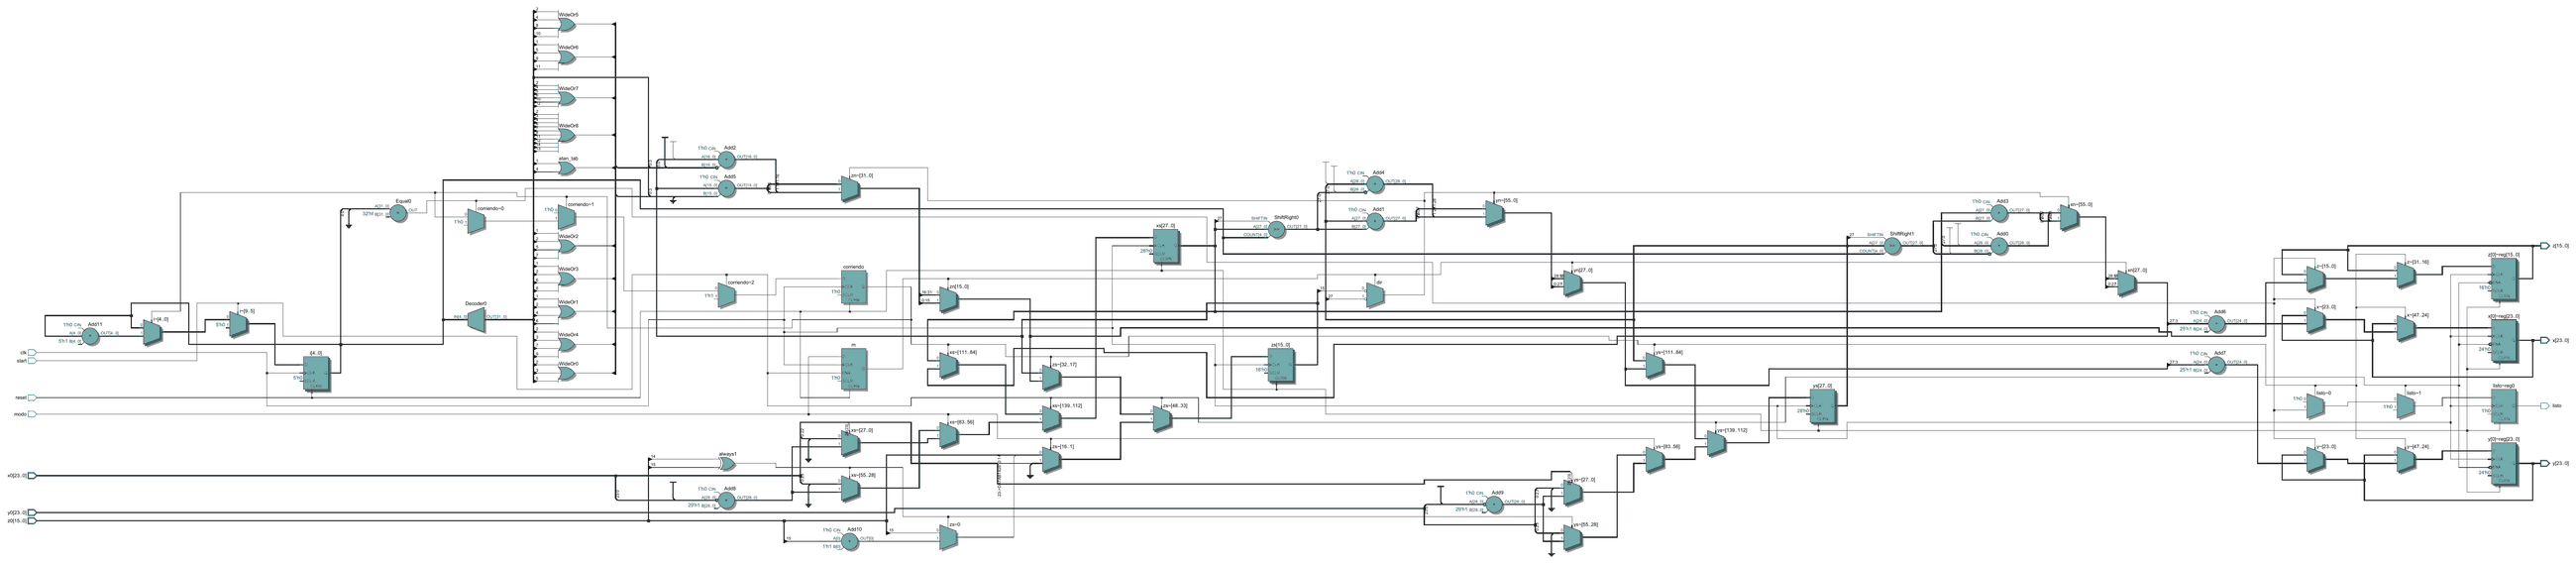
\includegraphics[width=\linewidth]{figs/rtl/rtl_cordic.png}
\caption{El módulo completo; a la izquierda, la tabla de arcotangentes.}
\end{subfigure}

\medskip
\begin{subfigure}{0.52\textwidth}
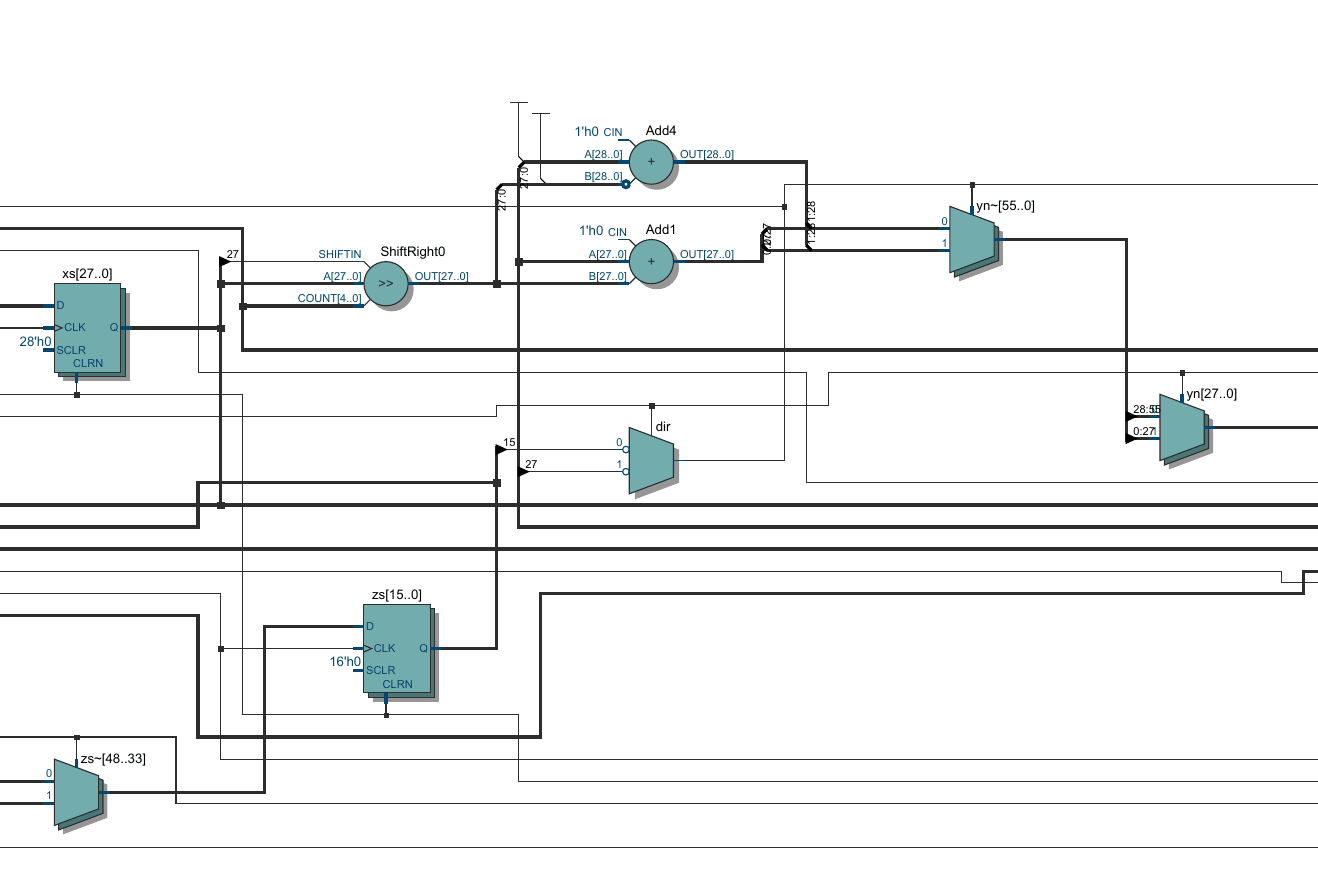
\includegraphics[width=\linewidth]{figs/rtl/zoom_cordic.png}
\caption{Acercamiento a una iteración: corrimiento de $x$, suma y resta, y el sentido de giro \sig{dir}.}
\end{subfigure}
\caption{\sig{cordic} en el RTL Viewer.}
\label{fig:rtlcordic}
\end{figure}

Nueve circuitos iguales, con $N$ de 4 a 20, recibieron los mismos 360 vectores y 360 ángulos
(figura~\ref{fig:cordiciter} y tabla~\ref{tab:cordiciter}). El error se divide entre cuatro cada dos iteraciones
hasta $N=14$ y ahí se estanca, porque la tabla de 16 bits se agota. Con $N=16$ el error máximo es de
0.017\textdegree, veinte veces menos que el paso de 0.35\textdegree{} con que el rumbo viaja por la red.
\sig{tb\_cordic} prueba además los cuatro cuadrantes y 200 divisiones: 248 de 248.

\begin{figure}[!htb]
\centering
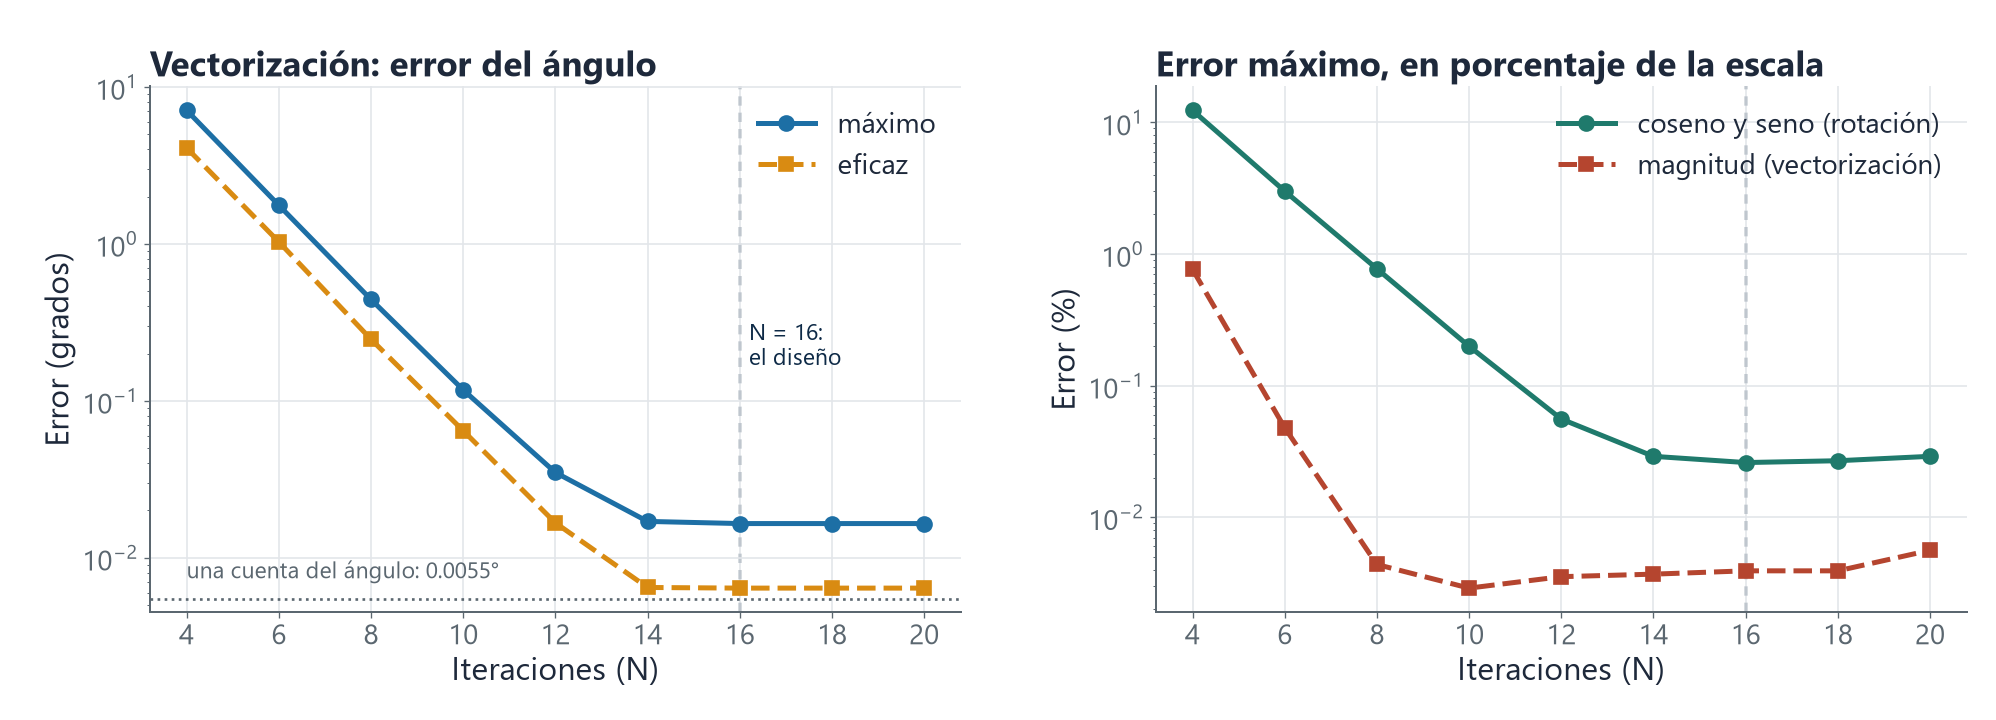
\includegraphics[width=0.96\textwidth]{figs/cordic_iteraciones.png}
\caption{Error del CORDIC según el número de iteraciones, medido en la simulación del circuito.}
\label{fig:cordiciter}
\end{figure}

\begin{table}[!htb]
\centering\footnotesize
\caption{Error máximo del CORDIC (\sig{tb\_cordic\_iter}).}
\label{tab:cordiciter}
\rowcolors{2}{SoftGray}{white}
\begin{tabularx}{0.86\textwidth}{@{}>{\bfseries}c >{\raggedleft\arraybackslash}X >{\raggedleft\arraybackslash}X >{\raggedleft\arraybackslash}X >{\raggedleft\arraybackslash}X@{}}
\toprule
\rowcolor{TableHead} $N$ & Ángulo (\textdegree) & Ángulo, eficaz (\textdegree) & Magnitud (\%) & Coseno y seno (\%) \\
\midrule
4  & 7.093 & 4.083 & 0.764 & 12.369 \\
8  & 0.442 & 0.246 & 0.0044 & 0.773 \\
12 & 0.035 & 0.017 & 0.0035 & 0.056 \\
16 & 0.017 & 0.0064 & 0.0039 & 0.026 \\
20 & 0.017 & 0.0064 & 0.0056 & 0.029 \\
\bottomrule
\end{tabularx}
\end{table}

\modulo{divisor\_u}{hdl/cordic.v}{84 a 195 EL}
Divisor con restauración: por ciclo baja un bit del dividendo al resto, prueba si cabe el divisor y, si cabe, lo
resta y pone un 1 en el cociente. Tarda un ciclo por bit más uno. La triangulación usa uno de 44 entre 32 bits y
el rumbo, uno de 20 entre 7.

\modulo{tri\_distancia}{hdl/tri\_red.v}{87 a 109 EL, 60 R}
\label{sec:raiz}%
Calcula $d=\lfloor\sqrt{\Delta x^2+\Delta y^2}\rfloor$ con la raíz dígito por dígito: baja dos bits del radicando
de 22 por ciclo, prueba si cabe $4q+1$ en el resto y, si cabe, lo resta y agrega un 1 a la raíz. En 12 ciclos da la
parte entera exacta. La regla del alcance usa la misma suma de cuadrados, $\Delta x^2+\Delta y^2<(16\times32)^2$,
así que la distancia que se muestra y el corte de los 32~m no pueden contradecirse (figura~\ref{fig:rtldist}).

\begin{figure}[!htb]
\centering
\begin{subfigure}{\textwidth}
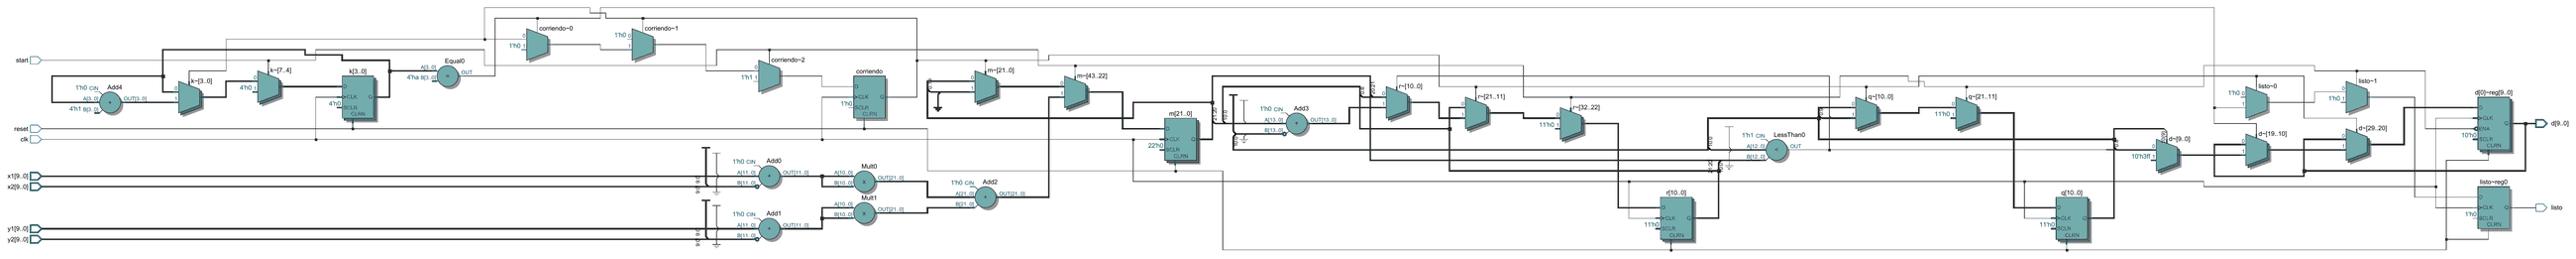
\includegraphics[width=\linewidth]{figs/rtl/rtl_tri_distancia.png}
\caption{El módulo completo.}
\end{subfigure}

\medskip
\begin{subfigure}{0.86\textwidth}
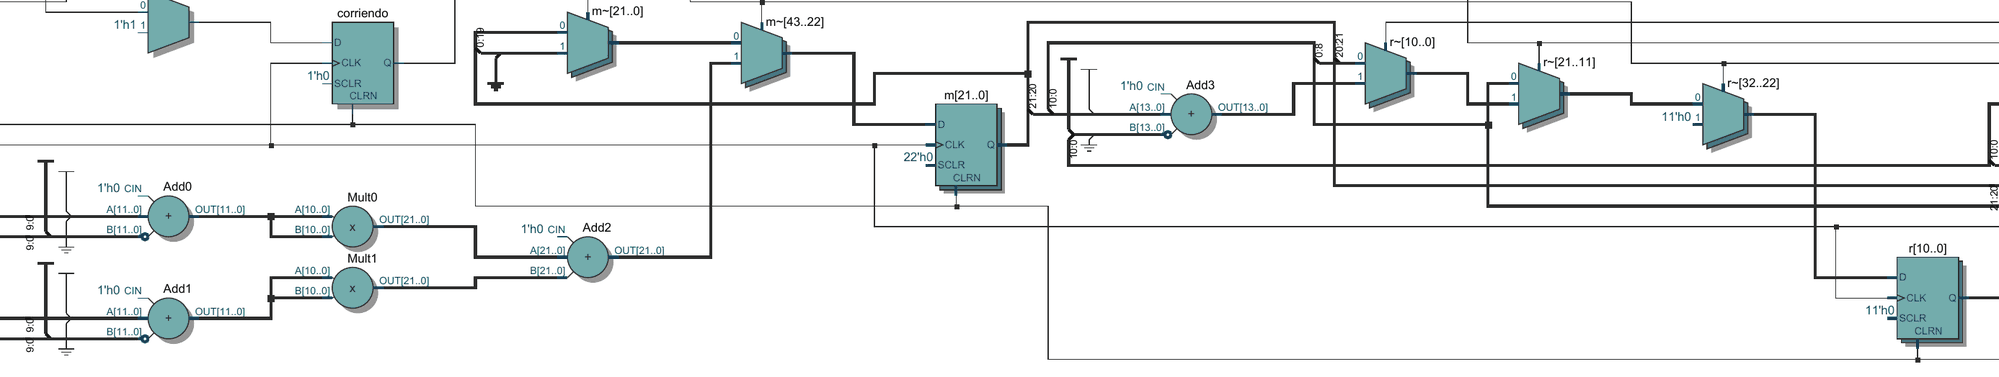
\includegraphics[width=\linewidth]{figs/rtl/zoom_tri_distancia.png}
\caption{Acercamiento: restas, los dos cuadrados (\sig{Mult0} y \sig{Mult1}), su suma y el registro del radicando.}
\end{subfigure}
\caption{\sig{tri\_distancia} en el RTL Viewer.}
\label{fig:rtldist}
\end{figure}

\textbf{FIR: media móvil.}\phantomsection\label{sec:fir} El filtro del núcleo es
$y[n]=\tfrac14(x[n]+x[n-1]+x[n-2]+x[n-3])$. No tiene realimentación, así que es estable, y su fase es lineal:
retrasa la señal un cuadro y medio sin deformarla. Con diez cuadros por segundo tiene nulos en 2.5 y 5~Hz
(figura~\ref{fig:filtros}, izquierda).

\modulo{tri\_tonos}{hdl/tonos.v}{355 EL, 225 R}
\label{sec:goertzel}%
Cada nodo emite un tono propio y escucha los otros dos: con saber a quién oye, sabe quién está a su alcance. El
micrófono, simulado como la suma de las ondas cuadradas que llegan más ruido, se muestrea a 16~kHz y cada 64
muestras (4~ms) tres filtros de Goertzel~\cite{goertzel1958} miden la potencia:
\begin{equation}
s[n]=x[n]+c\,s[n-1]-s[n-2],\qquad P=s[N_b-1]^2+s[N_b-2]^2-c\,s[N_b-1]\,s[N_b-2],
\end{equation}
con $c=2\cos(2\pi k/N_b)$. Los tonos de 1, 2 y 4~kHz caen en las líneas $k=4$, 8 y 16, de modo que uno no se cuela
en el filtro de otro; los coeficientes son 30\,274, 23\,170 y 0 en Q2.14. Un IIR con polos sobre el círculo
unitario podría acumular error, pero este corre 64 muestras y borra su estado. Un tono se da por oído si su
potencia pasa de 4\,000 en dos bloques seguidos y por perdido si queda debajo en dos: con el tono presente mide de
27\,000 a 33\,000 y sin él no pasa de 104 (figura~\ref{fig:filtros}, derecha). El tono propio sale por el pin~1 de
JP1, listo para un zumbador; con un micrófono real solo se sustituye la suma simulada.

\begin{figure}[!htb]
\centering
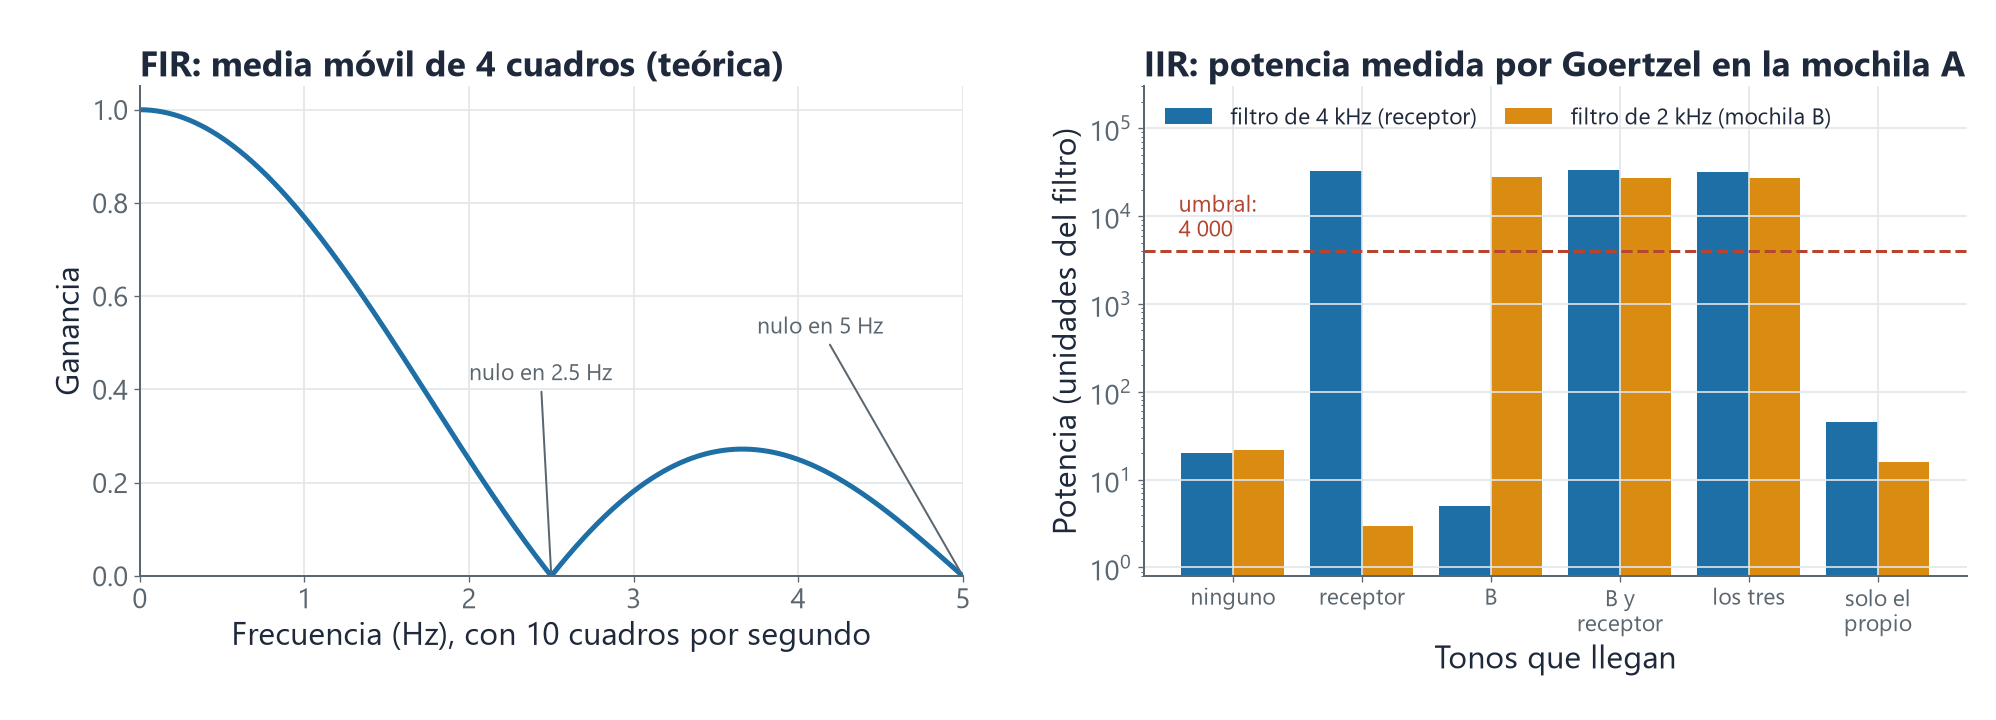
\includegraphics[width=0.97\textwidth]{figs/filtros.png}
\caption{Izquierda: respuesta de la media móvil (curva teórica). Derecha: potencia medida por los filtros de
Goertzel de la mochila A en la simulación del circuito (\sig{tb\_tonos}).}
\label{fig:filtros}
\end{figure}

\modulo{pid\_q}{hdl/pid\_q.v}{213 EL, 66 R, 79.96 MHz}
\label{sec:pid}%
PID en forma posicional, una muestra por pulso:
\begin{equation}
e[n]=r[n]-y[n],\qquad u[n]=K_p\,e[n]+K_i\sum_{k\le n}e[k]+K_d\,\bigl(e[n]-e[n-1]\bigr).
\end{equation}
El integral es un acumulador de 32 bits que guarda $K_i\sum e$ con sus ocho bits de fracción. La salida se satura
en $\pm U_{\max}$ y la saturación se decide con la suma completa de 40 bits. Si el actuador está en el tope y el
error empuja hacia el mismo lado, el acumulador se congela (integración condicional); un parámetro quita la
protección para compararla (figura~\ref{fig:rtlpid}). \sig{tb\_pid} cierra el lazo sobre $y[n+1]=y[n]+(4u[n]-y[n])/20$ junto a un PID en
aritmética real (figura~\ref{fig:pid}): la salida difiere en menos de una cuenta. El escalón de 200 tiene 9.3~\% de
sobrepaso y entra al 2~\% en 49 muestras; el de 1\,000, con el actuador saturado, 0.2~\% y 66 muestras, mientras
que sin protección la salida sigue en el tope 400 muestras después.

\begin{figure}[!htb]
\centering
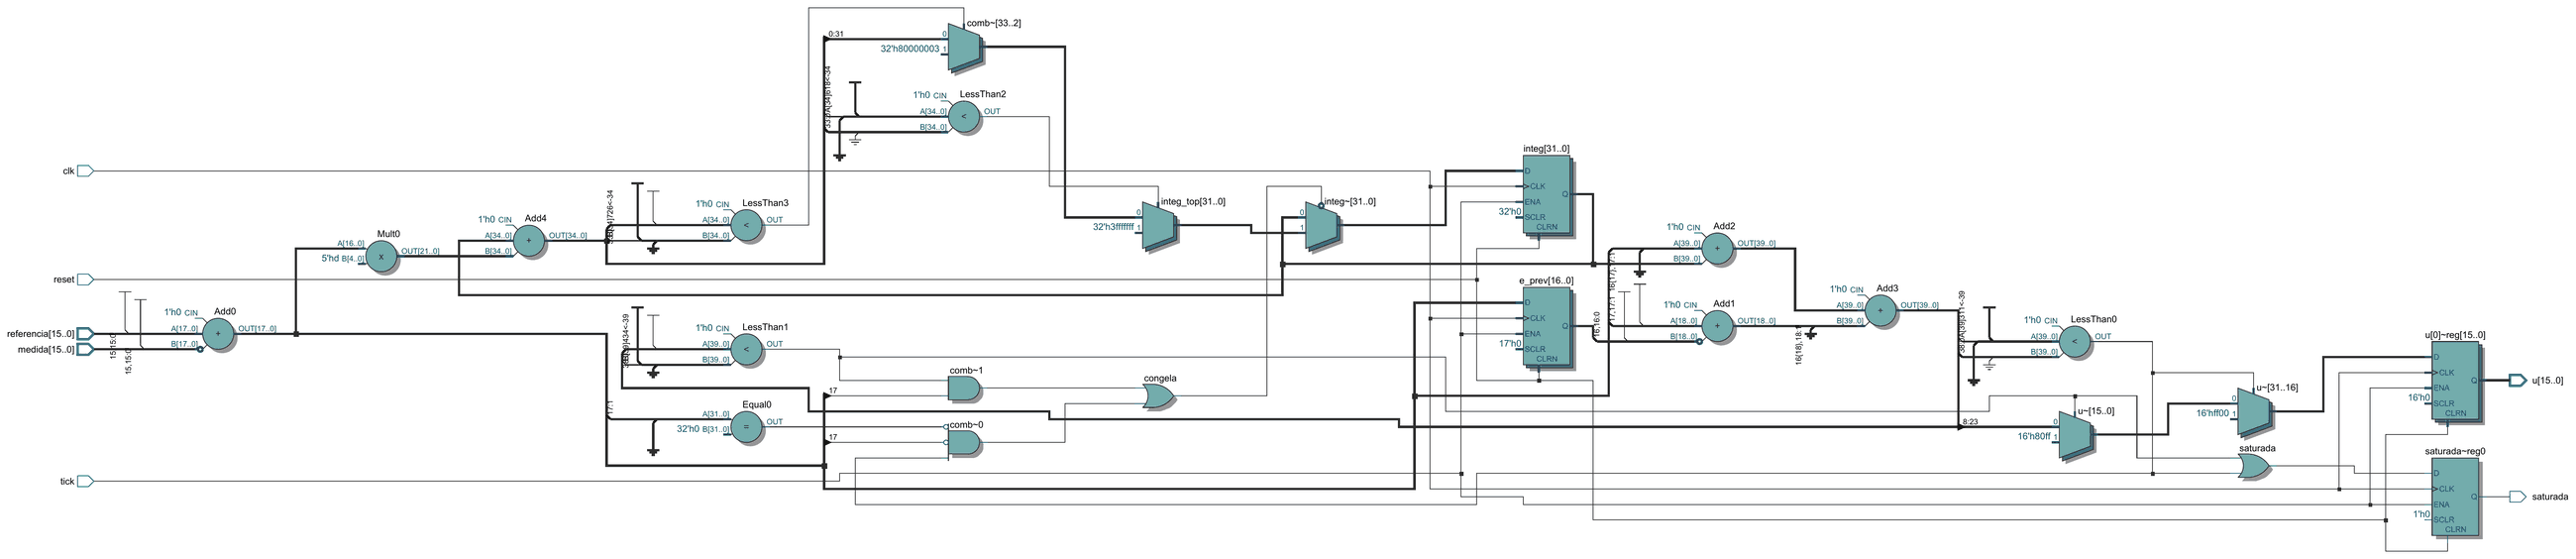
\includegraphics[width=\textwidth]{figs/rtl/rtl_pid_q.png}
\caption{\sig{pid\_q} en el RTL Viewer: error, producto integral, integrador con tope, congelamiento (\sig{congela}) y
saturación de la salida.}
\label{fig:rtlpid}
\end{figure}

\begin{figure}[!htb]
\centering
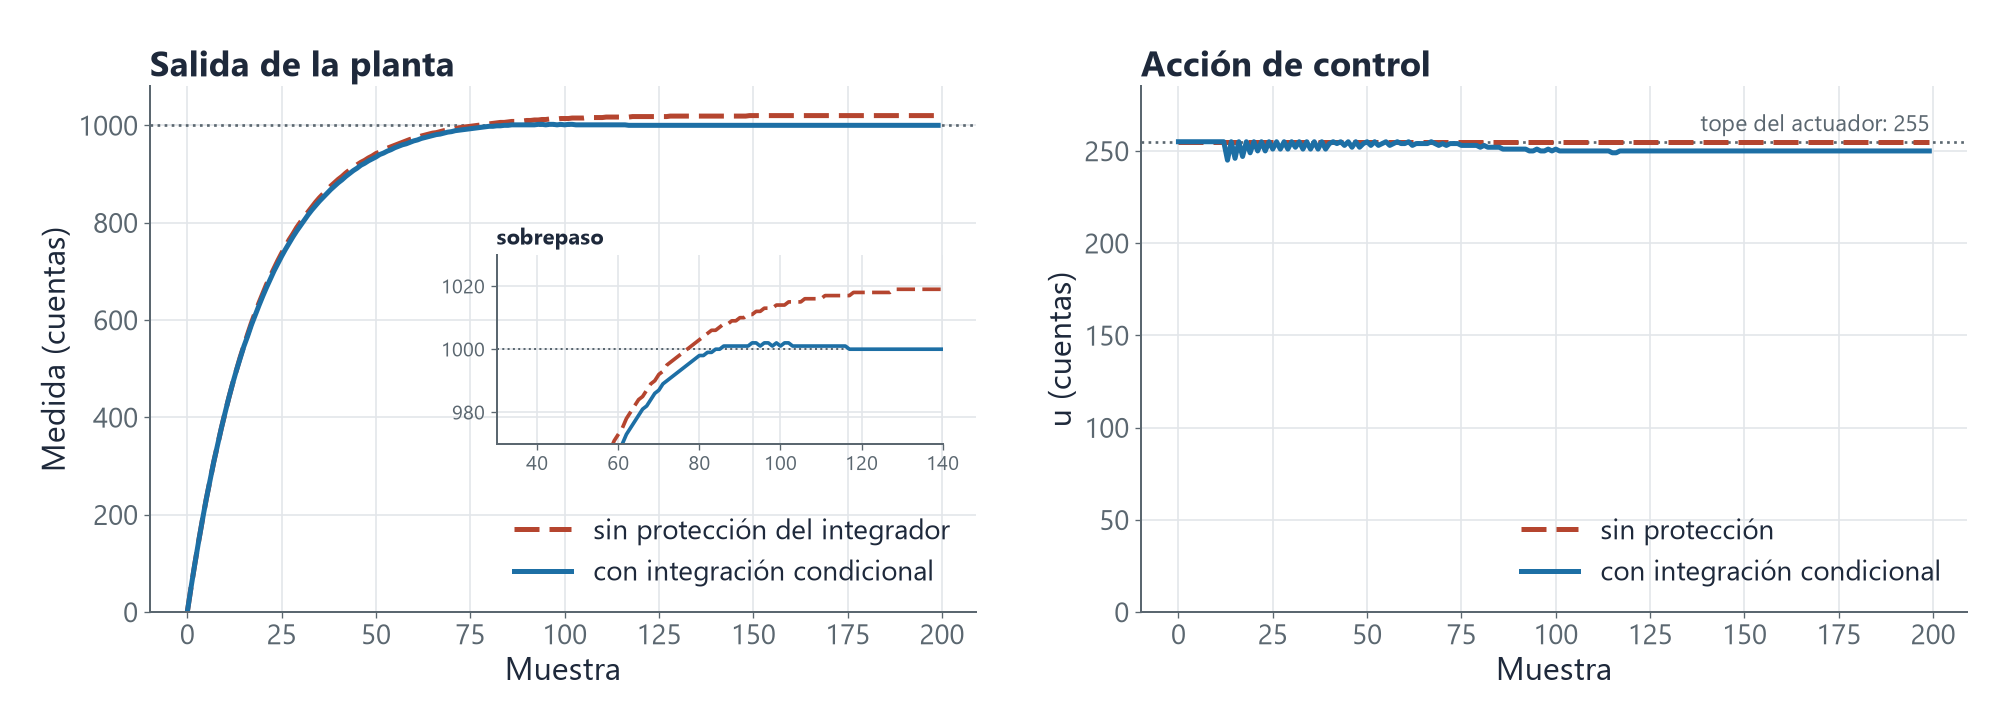
\includegraphics[width=0.86\textwidth]{figs/pid_respuesta.png}
\caption{Escalón de 1\,000 con el actuador saturado. Sin protección, la planta no vuelve a la referencia.}
\label{fig:pid}
\end{figure}

La búsqueda no usa un PID, porque su actuador es un pulso que el insecto obedece o no. Corresponde al modo de
regreso (sección~\ref{sec:regreso}): llevar a cero la diferencia entre dos fotodiodos que miran al faro, con la
tasa de estímulos como actuador. Ese modo no está en la demostración; aquí queda verificado con una planta de
prueba.

\subsection{Herramientas y procedimiento de verificación}
\label{sec:herramientas}

\begin{table}[H]
\centering\footnotesize
\caption{Herramientas del proyecto.}
\label{tab:herramientas}
\rowcolors{2}{SoftGray}{white}
\begin{tabularx}{\textwidth}{@{}>{\bfseries\raggedright\arraybackslash}p{4.4cm} >{\raggedright\arraybackslash}X@{}}
\toprule
\rowcolor{TableHead} Herramienta & Para qué se usó \\
\midrule
Python 3.12 & Simulación de la misión, modelo de referencia del núcleo y figuras \\
Icarus Verilog 12~\cite{icarus} & Simulación de todos los bancos de prueba \\
Active-HDL 17, edición estudiantil & Proyecto con todos los módulos y macros para ver las formas de onda \\
Quartus Prime Lite 24.1 & Síntesis, colocación, ruteo y análisis de tiempos para la MAX~10 \sig{10M50DAF484C7G} \\
DE10-Lite~\cite{terasic}, tres tarjetas & Pruebas en hardware: una, dos y tres tarjetas unidas por UART \\
Sonda de Quartus por JTAG~\cite{intelissp} & Leer los registros de las tarjetas y fijar sus entradas desde la computadora \\
LibreLane 3.0.17 con la PDK \sig{sky130A}~\cite{librelane,skywater} & Layout del núcleo, de RTL a GDS, en una máquina virtual con Ubuntu 24.04 \\
\bottomrule
\end{tabularx}
\end{table}

Cada bloque se verificó solo antes de conectarlo, en este orden:
\begin{enumerate}
  \item \textbf{Modelo de referencia.} Antes de escribir el Verilog del núcleo se programó en Python un
        modelo que hace las mismas cuentas con enteros, registro por registro. Ese modelo genera
        los cuadros de prueba y la respuesta esperada.
  \item \textbf{Bancos autoverificables.} Cada banco compara contra un valor esperado y termina con una
        línea de resultado; ninguno se revisa a ojo. Los bloques numéricos se comparan contra el
        valor exacto en aritmética real, y la distancia, contra todos los puntos del mapa.
  \item \textbf{Integración.} El banco \sig{tb\_tri} cablea las tres FPGA como en el laboratorio y recorre
        nueve escenarios; lee los displays y los LED como los vería una persona.
  \item \textbf{Síntesis y tiempos.} Las cuatro variantes de la red se compilan con el reloj de 50~MHz
        y se exige holgura positiva en el peor caso y cero advertencias críticas. Después de cada
        cambio se comparan los recursos con la síntesis anterior: una diferencia inesperada delata
        lógica eliminada.
  \item \textbf{Tarjetas.} Los mismos escenarios se repiten en las DE10-Lite fijando las entradas y
        leyendo los registros por la sonda de JTAG, sin instrumentos externos.
  \item \textbf{La terminal sin tarjetas.} Para probar el programa de la computadora cuando no hay
        tarjetas, sus funciones de JTAG se sustituyen por archivos y del otro lado se simulan las
        tres FPGA con sus módulos superiores: la orden que escribe el operador, los bits que llegan
        a la FPGA, lo que el circuito hace y lo que la terminal muestra se comprueban de corrido.
\end{enumerate}

\subsubsection{Flujo del layout}
\label{sec:flujo-layout}

El núcleo de la mochila, que es lo que iría en un circuito integrado, se pasó por el flujo
abierto completo de RTL a GDS con la PDK \sig{sky130A} de SkyWater~\cite{skywater} y la
biblioteca de celdas \sig{sky130\_fd\_sc\_hd}. La herramienta fue LibreLane 3.0.17~\cite{librelane},
el sucesor de OpenLane~\cite{shalan2020}: usa los mismos programas (Yosys para la síntesis,
OpenROAD para el plano, la colocación, el árbol de reloj y el ruteo, y Magic, Netgen y KLayout
para la verificación física) y el repositorio de OpenLane remite a él para diseños nuevos. La
entrada son los cinco archivos Verilog del núcleo, sin modificar.

La configuración tiene tres decisiones. El reloj es de 20~ns, el de 50~MHz de la tarjeta,
porque el generador de estímulo cuenta sus pulsos con esa frecuencia. La ocupación del núcleo
se pidió en 40~\% y la densidad de colocación en 55~\%, para rutear sin congestión. Y se activó
la reparación de transiciones lentas después del ruteo global, con márgenes de 50~\%: con los
valores por omisión la corrida pasaba DRC y LVS pero dejaba 140 transiciones de más de 0.75~ns
en la esquina lenta, causadas por los búferes débiles que agrega la reparación de \emph{hold};
con ese ajuste quedaron en cero. Los resultados están en la sección~\ref{sec:layout}.

